% =====================================================================
%  AURORA -- SYSC 4907 Project Proposal
%  Build:  latexmk -pdf main_short.tex      (pdflatex + bibtex)
%  Needs, in the same folder: team.tex, references.bib, f3_field_rates.dat
%  (the .dat is also looked for in figures/ and data/).
% =====================================================================
\documentclass[11pt,letterpaper]{article}

\usepackage[margin=1in,headheight=22pt]{geometry}
\usepackage[T1]{fontenc}
\usepackage[utf8]{inputenc}
\usepackage{lmodern}
\usepackage[scaled=0.92]{helvet}
\usepackage{microtype}
\usepackage[english]{babel}
\usepackage{setspace}
\setstretch{1.05}
\setlength{\parskip}{0.4em}
\setlength{\parindent}{0pt}

\usepackage{amsmath,amssymb,mathtools,bm}
\usepackage[per-mode=symbol]{siunitx}
\sisetup{group-separator={,},group-minimum-digits=4}
\DeclareSIUnit{\bar}{bar}
\DeclareSIUnit{\day}{d}
\usepackage{booktabs,tabularx,longtable,array,makecell}
\usepackage[table]{xcolor}
\renewcommand{\arraystretch}{1.12}
\newcolumntype{L}{>{\raggedright\arraybackslash}X}
\newcolumntype{P}[1]{>{\raggedright\arraybackslash}p{#1}}

\usepackage{graphicx}
\usepackage{tikz}
\usetikzlibrary{arrows.meta,positioning,shapes.geometric,shapes.misc,fit,backgrounds,calc,decorations.pathreplacing,shadows,matrix}
\usepackage{pgfplots}
\pgfplotsset{compat=1.18}
\usepgfplotslibrary{fillbetween}
\usepackage{pgfgantt}
\usepackage{adjustbox}
\usepackage{pdflscape}
\usepackage{pifont}
\usepackage{fontawesome5}
\usepackage{float}
\usepackage[section]{placeins}
\usepackage[font=small,labelfont={bf,sf},format=hang]{caption}
\setlength{\textfloatsep}{10pt plus 2pt minus 2pt}
\renewcommand{\topfraction}{0.9}
\renewcommand{\bottomfraction}{0.8}
\renewcommand{\textfraction}{0.07}
\renewcommand{\floatpagefraction}{0.8}
\setcounter{topnumber}{3}
\setcounter{totalnumber}{5}
\setlength{\intextsep}{8pt plus 2pt minus 2pt}

\definecolor{aurNavy}{HTML}{14213D}
\definecolor{aurBlue}{HTML}{2A6F97}
\definecolor{aurTeal}{HTML}{2A9D8F}
\definecolor{aurSand}{HTML}{E9C46A}
\definecolor{aurOrange}{HTML}{F4A261}
\definecolor{aurRed}{HTML}{C8553D}
\definecolor{aurGrey}{HTML}{6C757D}
\definecolor{aurLight}{HTML}{EEF3F7}
\definecolor{aurPurple}{HTML}{6D597A}
\colorlet{cIsmael}{aurBlue}
\colorlet{cAziz}{aurTeal}
\colorlet{cAbdu}{aurPurple}
\colorlet{cMahdi}{aurOrange}
\colorlet{cTimur}{aurRed}

\usepackage[explicit]{titlesec}
\titleformat{\section}{\sffamily\Large\bfseries\color{aurNavy}}
  {\thesection}{0.8em}{#1}[{\color{aurBlue}\titlerule[0.8pt]}]
\titleformat{\subsection}{\sffamily\large\bfseries\color{aurNavy}}
  {\thesubsection}{0.7em}{#1}
\titlespacing*{\section}{0pt}{1.1em}{0.6em}
\titlespacing*{\subsection}{0pt}{0.8em}{0.3em}

\usepackage{fancyhdr}
\pagestyle{fancy}
\fancyhf{}
\fancyhead[L]{\sffamily\footnotesize\color{aurGrey}AURORA \textbullet{} Project Proposal}
\fancyhead[R]{\sffamily\footnotesize\color{aurGrey}SYSC 4907}
\fancyfoot[C]{\sffamily\small\thepage}
\renewcommand{\headrulewidth}{0.4pt}

\usepackage{enumitem}
\setlist{itemsep=0.1em,topsep=0.2em,parsep=0pt}
\usepackage[most]{tcolorbox}
\newtcolorbox{keybox}[1][]{enhanced,colback=aurLight,colframe=aurBlue,
  boxrule=0pt,leftrule=3pt,arc=0pt,left=8pt,right=8pt,top=4pt,bottom=4pt,
  fonttitle=\sffamily\bfseries\color{aurNavy},coltitle=aurNavy,
  attach title to upper={\ },#1}

\newcommand{\tbc}[1]{\textcolor{aurOrange!85!black}{[#1]}}
\newcommand{\aur}{\textsc{Aurora}}
\newcommand{\cmark}{\textcolor{aurTeal}{\ding{51}}}
\newcommand{\pmark}{\textcolor{aurOrange}{$\circ$}}
\newcommand{\eg}{e.g.,\ }
\newcommand{\ie}{i.e.,\ }
\DeclareRobustCommand{\skilllead}{\tikz[baseline=-0.6ex]\fill[aurNavy] (0,0) circle (2.6pt);}
\DeclareRobustCommand{\skillsup}{\tikz[baseline=-0.6ex]\draw[aurNavy,thick] (0,0) circle (2.3pt);}

\usepackage[hidelinks]{hyperref}
\hypersetup{colorlinks=true,linkcolor=aurNavy,citecolor=aurBlue,urlcolor=aurBlue,
  pdftitle={AURORA -- Project Proposal},pdfauthor={AURORA Team},
  pdfsubject={SYSC 4907 Project Proposal}}
\usepackage[capitalise,noabbrev]{cleveref}
\usepackage{url}

\input{team}

% Locate the F3 rates file wherever the repository keeps it.
\newcommand{\FthreeData}{f3_field_rates.dat}
\IfFileExists{figures/f3_field_rates.dat}{\renewcommand{\FthreeData}{figures/f3_field_rates.dat}}{}
\IfFileExists{data/f3_field_rates.dat}{\renewcommand{\FthreeData}{data/f3_field_rates.dat}}{}

\begin{document}


% ---------------------------------------------------------------- Title
\begin{titlepage}
\centering
\vspace*{0.2cm}
{\sffamily\bfseries\fontsize{40}{44}\selectfont\color{aurNavy}AURORA\par}
\vspace{0.3cm}
{\sffamily\Large\color{aurBlue}Autonomous Upstream Reservoir Optimization and Risk-Aware Agent\par}
\vspace{0.6cm}
{\sffamily\LARGE\bfseries Project Proposal\par}
\vspace{0.3cm}
{\large Keeping an AI controller for an oil reservoir within its limits\\
when the model it relies on is wrong\par}
\vspace{0.7cm}
\begin{tabularx}{0.9\textwidth}{@{}P{2.6cm}L@{}}
\textbf{Course} & \CourseCode{} --- \CourseName, \Department, \University\\
\textbf{Supervisors} & \SupervisorA{} and \SupervisorB\\
\textbf{Submitted} & \SubmissionDate\\
\textbf{Repository} & \url{https://github.com/ismaelouadria/AURORA}\\
\end{tabularx}
\vspace{0.6cm}

\small
\begin{tabularx}{\textwidth}{@{}P{3.7cm}P{1.8cm}P{3.0cm}L@{}}
\toprule
\textbf{Name} & \textbf{Student no.} & \textbf{Program} & \textbf{Main responsibility}\\
\midrule
\Ismael & \IsmaelID & \IsmaelProg & Fast model, safety check, safety margin, overall design\\
\Aziz & \AzizID & \AzizProg & Detailed reservoir simulation (OPM Flow + Egg)\\
\Abdu & \AbduID & \AbduProg & AI controller (reinforcement learning)\\
\Mahdi & \MahdiID & \MahdiProg & Experiments, logging, statistics, dashboard, and result interpretation\\
\Timur & \TimurID & \TimurProg & Fault testing and failure handling\\
\bottomrule
\end{tabularx}
\normalsize
\vfill
\raggedright
\begin{keybox}[title=Summary.]
An AI controller decides how much water to pump into a simulated oil reservoir. Before each
decision is applied, a safety check uses a fast, simplified model to predict whether it
would push a well's pressure past its limit. If the model is wrong, a decision that looks safe can still break the limit. \aur{} measures
how wrong the fast model is by comparing it with a detailed simulator, turns that error
into a safety margin, and then tests, on reservoirs the system has never seen, whether the
margin reduces limit violations without giving up much oil production.
\end{keybox}
\end{titlepage}

% ============================================================== 1
\section{Introduction}

Oil is held in the tiny pores of underground rock. As oil is pumped out, the pressure in
the reservoir drops and production slows. \emph{Waterflooding} is a common way to keep
production going: water is pumped in through \emph{injector} wells, which keeps the
pressure up and pushes oil towards \emph{producer} wells. Someone has to decide, every few
weeks or months, how much water each injector should get (\cref{fig:waterflood}). That is
a control problem.

\begin{figure}[!htbp]
\centering
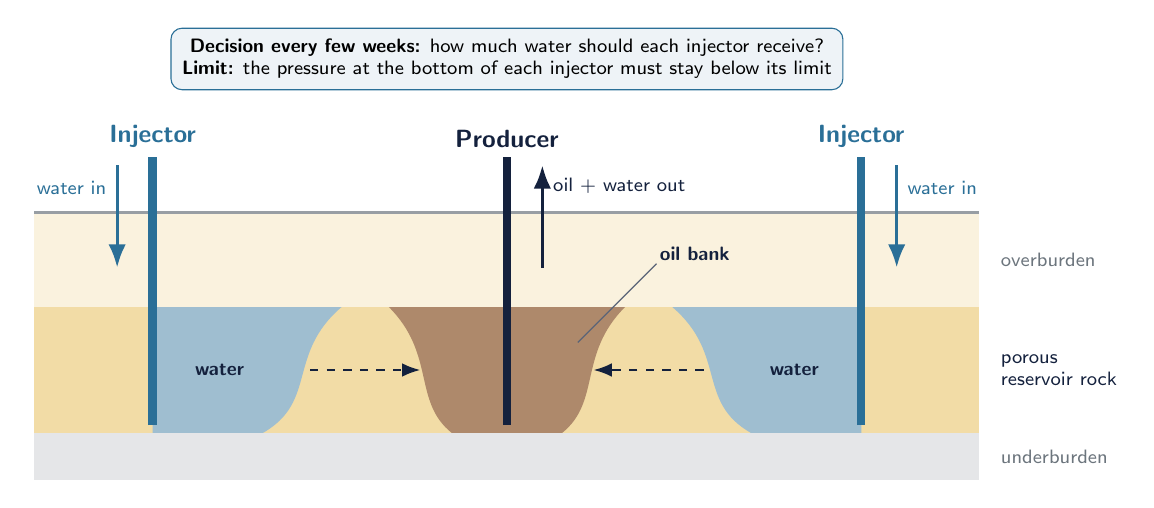
\begin{tikzpicture}[font=\sffamily\small,>=Latex]
  % layers
  \fill[aurSand!22] (0,2.2) rectangle (12,3.4);            % overburden
  \fill[aurSand!60] (0,0.6) rectangle (12,2.2);            % reservoir
  \fill[aurGrey!18] (0,0) rectangle (12,0.6);              % underburden
  \draw[aurGrey!70,thick] (0,3.4) -- (12,3.4);             % surface
  % fluids in the reservoir
  \fill[aurBlue!45] (1.5,0.6) -- (1.5,2.2) -- (3.9,2.2) .. controls (3.2,1.6) and (3.6,1.0) .. (2.9,0.6) -- cycle;
  \fill[aurBlue!45] (10.5,0.6) -- (10.5,2.2) -- (8.1,2.2) .. controls (8.8,1.6) and (8.4,1.0) .. (9.1,0.6) -- cycle;
  \fill[aurOrange!60!black!75] (4.5,2.2) .. controls (5.1,1.6) and (4.8,1.0) .. (5.3,0.6) -- (6.7,0.6) .. controls (7.2,1.0) and (6.9,1.6) .. (7.5,2.2) -- cycle;
  \draw[aurNavy!70] (6.9,1.75) -- (7.9,2.75) node[anchor=south west,inner sep=1pt,font=\sffamily\scriptsize\bfseries,text=aurNavy] {oil bank};
  \node[font=\sffamily\scriptsize\bfseries,text=aurNavy] at (2.35,1.4) {water};
  \node[font=\sffamily\scriptsize\bfseries,text=aurNavy] at (9.65,1.4) {water};
  % displacement arrows
  \draw[->,thick,aurNavy,dashed] (3.5,1.4) -- (4.9,1.4);
  \draw[->,thick,aurNavy,dashed] (8.5,1.4) -- (7.1,1.4);
  % wells
  \foreach \x/\lab/\col in {1.5/Injector/aurBlue, 10.5/Injector/aurBlue, 6.0/Producer/aurNavy}{
    \draw[line width=3pt,\col] (\x,0.7) -- (\x,4.1);
    \node[above,font=\sffamily\small\bfseries,text=\col] at (\x,4.1) {\lab};}
  \draw[->,very thick,aurBlue] (1.05,4.0) -- node[pos=0.22,left,font=\sffamily\scriptsize,text=aurBlue]{water in} (1.05,2.7);
  \draw[->,very thick,aurBlue] (10.95,4.0) -- node[pos=0.22,right,font=\sffamily\scriptsize,text=aurBlue]{water in} (10.95,2.7);
  \draw[->,very thick,aurNavy] (6.45,2.7) -- node[pos=0.8,right,font=\sffamily\scriptsize,text=aurNavy]{oil + water out} (6.45,4.0);
  % layer labels (outside the drawing)
  \node[font=\sffamily\scriptsize,text=aurGrey,anchor=west] at (12.15,2.8) {overburden};
  \node[font=\sffamily\scriptsize,text=aurNavy,anchor=west,align=left] at (12.15,1.4) {porous\\reservoir rock};
  \node[font=\sffamily\scriptsize,text=aurGrey,anchor=west] at (12.15,0.3) {underburden};
  % decision annotation
  \node[draw=aurBlue,fill=aurLight,rounded corners,font=\sffamily\scriptsize,align=center,inner sep=4pt]
     at (6.0,5.35) {\textbf{Decision every few weeks:} how much water should each injector receive?\\
     \textbf{Limit:} the pressure at the bottom of each injector must stay below its limit};
\end{tikzpicture}
\caption[Conceptual waterflood]{How a waterflood works. Injectors push water through the reservoir towards a
producer. The decision to make is how much water each injector pumps over time.}
\label{fig:waterflood}
\end{figure}

Three things make it hard:
\begin{itemize}
\item \textbf{Limited view.} Nobody can see what is happening underground. The only
measurements come from the wells: flow rates, the fraction of produced liquid that is water
(the \emph{water cut}), and the pressure at the bottom of each well (\emph{bottom-hole
pressure}, BHP).
\item \textbf{Delayed effects.} Pumping more water today can raise production now but cause
water to reach the producers sooner, which lowers the total oil recovered.
\item \textbf{Slow or inaccurate models.} A detailed simulator is accurate but too slow to
run for every decision being considered. A fast simplified model is quick but wrong by an
unknown amount.
\end{itemize}

Reinforcement learning (RL), where a program learns good decisions by trial and error in a
simulator, has been used for waterflooding several times
\cite{hourfar2019rl,ma2019drl,zhang2022drl}. Giving the controller a memory of past
measurements is the usual way to deal with the limited view
\cite{kaelbling1998pomdp,hausknecht2015drqn}. However, an RL controller only tries to
maximize its score. Nothing guarantees that each decision respects operating limits
\cite{garcia2015survey}. The usual fix is a \emph{safety filter}: a check placed between
the controller and the reservoir. It predicts the effect of each proposed decision and, if
a limit would be broken, replaces the decision with the closest safe one
\cite{wabersich2021filter}.

\begin{keybox}[title=The problem this project addresses.]
A safety filter can only catch what its model predicts. Suppose the pressure limit for an
injector is \SI{420}{\bar} and the fast model predicts \SI{414}{\bar} for a proposed
decision. The filter lets it through. If the detailed simulator then gives \SI{423}{\bar},
the limit is broken even though the filter worked as designed. The fast model was wrong,
and nothing in the system allowed for that.
\end{keybox}

\aur{} treats the error of the fast model as part of the safety problem. It measures that
error against the detailed simulator, focusing on the cases where the fast model predicts
too low, and adds a safety margin of a size the measurements justify.

\textbf{Scope.} This is a software and computer engineering project that uses an oil
reservoir as its application. The work is software design, connecting to an existing
simulator, machine learning, optimization, statistics, testing, failure handling and
visualization. Everything is tested in simulation, using a published test reservoir (the
Egg model \cite{jansen2014egg}) in an open-source simulator (OPM Flow
\cite{rasmussen2021opm}). We do not claim the system is ready for a real oil field, nor 
that our system surpasses those currently used in practice.

% ============================================================== 2
\section{Objectives and Requirements}\label{sec:req}

\subsection{Objectives}

\textbf{Main objective.} Build and test a software system that (1) controls water injection
in a simulated reservoir using an RL controller with memory, (2) protects a pressure limit
with a safety filter based on a fast model, and (3) finds out whether adding a margin based
on the fast model's measured error reduces limit violations on reservoirs the system has
not seen before.

Each supporting objective has one owner, so it is clear who is responsible for it
(\cref{tab:objectives}).

\begin{table}[!htbp]
\caption{Supporting objectives, owners and how we show each one is done.}\label{tab:objectives}
\small
\begin{tabularx}{\textwidth}{@{}lLP{2.1cm}P{5.0cm}@{}}
\toprule
\textbf{ID} & \textbf{Objective} & \textbf{Owner} & \textbf{Shown by}\\
\midrule
O1 & Detailed simulation that our software can drive step by step: any Egg reservoir version running in OPM Flow & \AzizS & Runs from a fresh copy of the repository with one script; tests on the extracted data\\
O2 & AI controller that sees only well measurements, in two forms: without memory (PPO) and with memory (recurrent PPO) & \AbduS & Saved settings and random seeds; a test proving no hidden data reaches the controller\\
O3 & Fast model fitted to each reservoir version, and a safety filter that changes unsafe decisions as little as possible & \IsmaelS & Report comparing the fast model with OPM; unit tests for the filter\\
O4 & Measurement of the fast model's error and a safety margin built from it & \IsmaelS, \AzizS & Dataset of paired fast-model and OPM results; report on how well the margin covers the error\\
O5 & Fault testing and a supervisor that falls back to a safe action when something fails & \TimurS & Library of fault scenarios; tests of the supervisor\\
O6 & Logging, an experiment runner, statistics and a dashboard & \MahdiS & A result figure regenerated from its saved run record\\
O7 & Test of the complete system on unseen reservoir versions & Team & Test plan fixed in advance; results with confidence intervals\\
\bottomrule
\end{tabularx}
\end{table}

\subsection{Functional requirements}

Every requirement is written so that it can be checked. Each has a priority
(\textbf{M}ust, \textbf{S}hould, \textbf{C}ould), an owner and a way of checking it
(T = automated test, E = experiment, D = demonstration, I = inspection). Values marked
\emph{proposed} are fixed at the design review and changed afterwards only through a
recorded decision.

{\small
\begin{longtable}{@{}P{1.1cm}P{9.4cm}P{0.5cm}P{2.1cm}P{0.7cm}@{}}
\caption{Functional requirements.}\label{tab:fr}\\
\toprule
\textbf{ID} & \textbf{The system shall\ldots} & \textbf{Pr.} & \textbf{Owner} & \textbf{Ver.} \\
\midrule
\endfirsthead
\toprule
\textbf{ID} & \textbf{The system shall\ldots} & \textbf{Pr.} & \textbf{Owner} & \textbf{Ver.} \\
\midrule
\endhead
\bottomrule
\endfoot
\multicolumn{5}{@{}l}{\sffamily\bfseries\color{aurNavy} Reservoir simulation} \\*
FR-01 & run any chosen Egg reservoir version in OPM Flow from settings kept under version control. & M & \AzizS & T \\
FR-02 & move the simulation forward one decision step at a time, applying injection rates supplied by our software. & M & \AzizS & T \\
FR-03 & after each step, read out well rates, total volumes, injector and producer BHP, and the pressure and water content of each cell, and save them in a fixed format. & M & \AzizS & T \\
FR-04 & check that the rates OPM applied equal the rates requested, and flag any difference. & M & \AzizS & T \\
FR-05 & produce matching fast-model and OPM results (same situation, same decision) for measuring the fast model's error. & M & \AzizS, \IsmaelS & T, E \\
\multicolumn{5}{@{}l}{\sffamily\bfseries\color{aurNavy} AI controller} \\*
FR-06 & provide the simulation through the Gymnasium interface, with documented observations and actions. & M & \AbduS & T \\
FR-07 & give the controller only well measurements it is allowed to see; an automated check rejects any hidden simulator data. & M & \AbduS & T \\
FR-08 & train and test controllers with and without memory from settings files, with the random seeds recorded. & M & \AbduS & E \\
FR-09 & provide a fixed-rate controller and a simple rule-based controller as baselines, connected in the same way as the learned controllers. & M & \AbduS & T \\
\multicolumn{5}{@{}l}{\sffamily\bfseries\color{aurNavy} Fast model and safety filter} \\*
FR-10 & fit the fast model (CRM) to the injection and production data of a given reservoir version, and predict the response to a candidate decision one step ahead. & M & \IsmaelS & T, E \\
FR-11 & solve the safety filter's optimization problem (\cref{eq:qp}) for every proposed decision and output the applied decision, the size of the change and which limit caused it. & M & \IsmaelS & T \\
FR-12 & detect when no safe decision exists and apply the documented fallback. & M & \IsmaelS, \TimurS & T \\
FR-13 & compute the fast model's errors and the safety margin from the margin (calibration) reservoirs only. & M & \IsmaelS & T, E \\
FR-14 & run the safety filter with no margin, a fixed margin or the measured margin, chosen in the settings. & M & \IsmaelS & T \\
\multicolumn{5}{@{}l}{\sffamily\bfseries\color{aurNavy} Failure handling} \\*
FR-15 & create repeatable faults on demand: missing, frozen, delayed, noisy or invalid measurements; a drifting fast model; controller or solver faults; a failed simulator step. & M & \TimurS & T \\
FR-16 & check each measurement (format, range, being a real number, how recent it is) before it reaches the controller. & M & \TimurS & T \\
FR-17 & detect a part that does not answer in time, and switch to a degraded or fallback mode with a limited, logged response. & M & \TimurS & T \\
FR-18 & record every fault, detection and change of mode in the logs. & M & \TimurS, \MahdiS & T \\
\multicolumn{5}{@{}l}{\sffamily\bfseries\color{aurNavy} Logging, experiments and presentation} \\*
FR-19 & log, for each decision step, the observation, proposed decision, applied decision, fast-model prediction, margin, result and supervisor mode, with each stage kept separate. & M & \MahdiS & T \\
FR-20 & save a record of every run (code version, settings, reservoir version, seeds, simulator version, fingerprints of the input files). & M & \MahdiS & T \\
FR-21 & run every combination of controller, reservoir version and seed in a batch, and keep failed runs together with the reason they failed. & M & \MahdiS & T, E \\
FR-22 & compute the final-test measurements, with confidence intervals, from the logged runs. & M & \MahdiS & T, E \\
FR-23 & replay any logged run in a dashboard and compare controllers visually. & M & \MahdiS & D \\
FR-24 & let a presenter trigger a fault scenario in the dashboard and show the supervisor's response. & S & \TimurS, \MahdiS & D \\
FR-25 & fit the CRM to the Volve production data, tested on the last part of each record, as a check against a real field. & S & \IsmaelS & E \\
FR-26 & support, for comparison, an RL controller trained to respect limits by itself. & C & \AbduS & E \\
\end{longtable}
}

\subsection{Non-functional requirements}

\begin{table}[H]
\caption{Non-functional requirements with measurable targets.}\label{tab:nfr}
\small
\begin{tabularx}{\textwidth}{@{}P{1.35cm}P{2.3cm}LP{0.7cm}@{}}
\toprule
\textbf{ID} & \textbf{Quality} & \textbf{Requirement and target} & \textbf{Ver.} \\
\midrule
NFR-01 & Reproducibility & A new team member can get a verified OPM run from a fresh copy of the repository using only the written steps; the simulator runs in a container with a fixed version. & D \\
NFR-02 & Reproducibility & Parts with no randomness give identical decisions for identical inputs; results of trained controllers repeat within the variation reported between seeds. & T \\
NFR-03 & Speed & \emph{Proposed:} controller, fast model and filter together take under \SI{1}{\second} per decision on a team laptop; the filter alone has a median time under \SI{50}{\milli\second}. & T \\
NFR-04 & Scaling up & The batch runner uses all available processor cores without changing the results. & T \\
NFR-05 & Testing & Unit tests cover at least 80\% of the lines in the safety, margin, supervisor and logging packages. & T \\
NFR-06 & Fair testing & The reservoir versions kept for the final test are fixed and recorded in advance; no training, margin or tuning job may read them, and any attempt is logged. & T, I \\
NFR-07 & Logging & Every decision step produces a complete log record; a missing field fails the run. & T \\
NFR-08 & Failure handling & Under every fault we test, no invalid or out-of-range decision reaches the simulator. & T \\
NFR-09 & Maintainability & Every package has a documented interface; every important design choice has a short written decision record. & I \\
NFR-10 & Ease of use & A second reader can understand the dashboard's main view without reading code, checked in a rehearsal with someone outside the team. & D \\
NFR-11 & Portability & Runs on Linux and macOS with Docker; automated tests run on GitHub Actions. & T \\
NFR-12 & Licensing & Equinor's licence terms and credit for the Volve data are respected. & I \\
\bottomrule
\end{tabularx}
\end{table}

\subsection{Use cases}

\Cref{fig:usecase} shows who uses the system and for what. The users are the
\emph{experimenter} (any team member running the system) and the \emph{reviewer}
(supervisors, second reader or poster-fair visitor). The OPM Flow simulator is an external
system. The three use cases at the heart of the project are UC1 (run a full simulation
with the controller in the loop), UC4 (compute the safety margin from the matching runs)
and UC6 (trigger a fault and observe the response). Their step-by-step descriptions are
kept in the repository.

\begin{figure}[!htbp]
\centering
\begin{adjustbox}{max width=\textwidth}
\begin{tikzpicture}[font=\sffamily\small,
  uc/.style={rounded rectangle,draw=aurBlue,fill=aurLight,thick,minimum width=5.3cm,minimum height=0.62cm,inner sep=2pt,align=center,font=\sffamily\footnotesize},
  opmuc/.style={uc,draw=aurTeal,fill=aurTeal!12},
  actor/.style={align=center,font=\sffamily\footnotesize\bfseries,text=aurNavy},
  inc/.style={aurGrey,dashed,->,thick},
  inclbl/.style={font=\sffamily\scriptsize,text=aurGrey}]
  \node[draw=aurNavy,rounded corners,thick,minimum width=12.4cm,minimum height=8.3cm] (sys) at (7.6,-3.05) {};
  \node[anchor=north,font=\sffamily\small\bfseries,text=aurNavy] at (sys.north) {AURORA system boundary};
  % left column: experimenter use cases
  \node[opmuc] (u1)  at (4.95,-0.1) {UC1 Run a full simulation with the controller};
  \node[uc]    (u2)  at (4.95,-1.2) {UC2 Train controller};
  \node[opmuc] (u3)  at (4.95,-2.3) {UC3 Produce matching fast-model/OPM data};
  \node[uc]    (u4)  at (4.95,-3.4) {UC4 Compute the safety margin};
  \node[opmuc] (u5)  at (4.95,-4.5) {UC5 Run a batch of experiments};
  \node[uc]    (u7)  at (4.95,-5.6) {UC7 Reproduce a result from its run record};
  \node[uc]    (u10) at (4.95,-6.7) {UC10 Fit CRM to Volve data};
  % right column: shared with reviewers
  \node[uc] (u6) at (10.9,-1.2) {UC6 Inject fault scenario};
  \node[uc] (u8) at (10.9,-3.4) {UC8 Replay and inspect run};
  \node[uc] (u9) at (10.9,-4.5) {UC9 Compare controllers};
  % actors
  \node[actor] (exp) at (-0.4,-2.3) {\Large\faUser\\[2pt]Experimenter\\(team member)};
  \node[actor,text=aurTeal] (opm) at (-0.4,-6.0) {\Large\faServer\\[2pt]OPM Flow\\simulator};
  \node[actor] (rev) at (15.6,-2.8) {\Large\faUserTie\\[2pt]Reviewer\\(supervisor, second\\reader, visitor)};
  % associations
  \foreach \u in {u1,u2,u3,u4,u5,u7,u10}{\draw[aurNavy!60] ([xshift=2pt]exp.east) -- (\u.west);}
  \foreach \u in {u1,u3,u5}{\draw[aurTeal,dashed,thick] ([xshift=2pt]opm.east) -- (\u.west);}
  \foreach \u in {u6,u8,u9}{\draw[aurNavy!60] ([xshift=-2pt]rev.west) -- (\u.east);}
  % include relations
  \draw[inc] ([xshift=1.3cm]u4.north) -- ([xshift=1.3cm]u3.south) node[midway,right,inclbl]{$\langle\!\langle$include$\rangle\!\rangle$};
  \draw[inc] (u9.west) -- node[above,inclbl]{$\langle\!\langle$include$\rangle\!\rangle$} (u5.east);
  % legend
  \node[anchor=north west,font=\sffamily\scriptsize,text=aurGrey,align=left] at ([yshift=-4pt]sys.south west)
    {\tikz[baseline=-0.6ex]\node[rounded rectangle,draw=aurTeal,fill=aurTeal!12,thick,minimum width=0.8cm,minimum height=0.3cm]{};\;
     Use case that runs the external OPM Flow simulator.\\
     The experimenter can also perform UC6, UC8 and UC9.};
\end{tikzpicture}
\end{adjustbox}
\caption[Use-case diagram]{Use-case diagram. Solid lines join each user to their main use cases; dashed teal lines
mark use cases that run the external OPM Flow simulator.}
\label{fig:usecase}
\end{figure}

% This part kind of sucks and needs to be review thoroughly
% \subsection{Success criteria and how progress is measured}

% Success is judged in two ways. The \emph{engineering criteria} are about building a system
% that works and can be checked. We expect to meet all of them:
% \begin{itemize}
% \item[E1] A complete simulation runs from start to finish with no manual steps, and every step is logged.
% \item[E2] Re-running a saved run record reproduces the same decisions.
% \item[E3] The safety filter never breaks its own limit when a safe decision exists, and always reports when none exists.
% \item[E4] Every fault scenario produces the response it was designed to produce.
% \item[E5] A reviewer can replay a run and see what the controller proposed, what was applied, why it was changed and what happened.
% \end{itemize}

% The \emph{research criteria} are the hypotheses in \cref{sec:eval}. The experiment may
% support them or not. A clear ``no, it did not help'', backed by evidence, still meets the
% project's objectives. All numeric thresholds are fixed before the final test.

% \textbf{Progress} is measured by what has been delivered, not by hours spent. Each
% milestone in \cref{sec:schedule} ends with something that can be shown: merged code,
% passing tests and saved results. Week to week, the team tracks milestones reached, open
% blockers, whether automated tests pass, and how many runs can be reproduced.

% \textbf{Not part of this project.} Use on a real oil field; any claim that the system is
% safe in the real world; inventing a new learning algorithm, fast model or statistical
% method (the contribution is combining existing ones and testing the combination); and
% treating simulator output as if it were reality.

% ============================================================== 3
\section{Background and State of the Art}

\textbf{Reservoir simulation and the Egg model.} A detailed (``full-physics'') reservoir
simulator divides the reservoir into thousands of small cells and solves the flow equations
for oil and water in each one. OPM Flow is an open-source simulator of this kind that reads
the standard input files used in industry \cite{rasmussen2021opm}. The Egg model
\cite{jansen2014egg,egg2014dataset} is a small made-up reservoir published for research on
waterflooding. It has eight injectors and four producers, about 18,500 cells, and a
simulated life of 3,600 days. It comes in 100 versions that differ in how easily fluid
flows through different parts of the rock, which represents not knowing the true geology.
Earlier work optimized injection on such models with gradient-based methods
\cite{brouwer2004dynamic}. These are accurate but slow, and must be redone whenever the
reservoir model changes.

\textbf{Fast models (CRM).} The capacitance--resistance model (CRM) describes a reservoir
as a set of connections between injectors and producers. Each connection responds to a
change in injection gradually, like a resistor--capacitor circuit
\cite{yousef2006crm,sayarpour2009crm}. Its settings are fitted from injection and
production data only, and it runs in microseconds where a detailed simulation takes
minutes. CRM is widely used for forecasting \cite{soroush2018crmreview}. It is known to be
less accurate when the rock varies a lot from place to place \cite{mamghaderi2021crm}, and
Egg is built to vary in exactly that way. We therefore expect the fast model to be wrong,
and the project is built around that.

\textbf{Reinforcement learning with a limited view.} When a controller cannot see the full
state of the system, the best decision depends on what it has seen in the past
\cite{kaelbling1998pomdp}. Proximal Policy Optimization (PPO) \cite{schulman2017ppo} is a
widely used RL algorithm. \emph{Recurrent} PPO adds a memory unit (an LSTM
\cite{hochreiter1997lstm}) so that the controller can remember earlier measurements. Both
are available in the open-source library Stable-Baselines3 \cite{raffin2021sb3}, which
uses the standard Gymnasium interface between a controller and a simulation
\cite{towers2024gymnasium}.

\textbf{Safety filters.} A safety filter changes unsafe decisions before they are applied
\cite{wabersich2021filter,dalal2018safety}. When the predicted effect of a decision is a
straight-line function of the decision, finding the closest safe decision is a small
optimization problem called a quadratic program (QP). Solvers such as OSQP handle it in
milliseconds \cite{stellato2020osqp}. Other approaches teach the controller the limits
during training instead \cite{achiam2017cpo}; one was recently applied to waterflooding
\cite{chen2025wcsac}.

\textbf{Measuring how wrong a model is.} \emph{Conformal prediction} is a simple
statistical method for putting a bound on a model's error. The model's errors are measured
on data set aside for that purpose, and a chosen percentile of those errors (for example
the 95th) is used as the bound. If new cases are similar to the ones measured, the bound
holds about that often \cite{lei2018conformal,angelopoulos2021gentle}. A one-sided version
looks only at errors in the dangerous direction. Versions that adapt over time exist for
data that change \cite{gibbs2021aci}.

\textbf{What is missing.} We searched the literature specifically for work that would make
this project unnecessary. Each piece exists already: RL for waterflooding, RL with safety
limits for waterflooding \cite{chen2025wcsac}, CRM and studies of its error
\cite{mamghaderi2021crm}, safety filters, and conformal prediction. In what we reviewed, we
did not find them put together the way \aur{} does: measuring the fast model's error
against a detailed simulator, turning the dangerous part of that error into a margin inside
a safety filter, and testing the result on reservoir versions never used during
development. Our contribution is that combination and a fair experiment that shows whether
it helps. Any potential similar projects may exist internally for company use, but none are 
released or open source.

% I really don't think we need this, this seems like extra BS
% \Cref{tab:related} compares the closest earlier work with the features that together
% define what \aur{} does.

% \begin{table}[!htbp]
% \centering\footnotesize
% \setlength{\tabcolsep}{3pt}
% \caption{Closest earlier work compared with the features of \aur{}. \cmark{} = present,
% \pmark{} = partly present or in a different form, blank = absent.}
% \label{tab:related}
% \begin{tabularx}{\textwidth}{@{}Lcccccccc@{}}
% \toprule
%  & \rotatebox{90}{\makecell[l]{Waterflood\\application}} & \rotatebox{90}{\makecell[l]{Limited\\view}} & \rotatebox{90}{\makecell[l]{Controller\\with memory}} & \rotatebox{90}{\makecell[l]{Physical fast\\model (CRM)}} & \rotatebox{90}{\makecell[l]{Filter that corrects\\each decision}} & \rotatebox{90}{\makecell[l]{Fast-model error\\measured}} & \rotatebox{90}{\makecell[l]{Margin from\\measured error}} & \rotatebox{90}{\makecell[l]{Safety tested on\\unseen reservoirs}} \\
% \midrule
% RL for waterflooding \cite{hourfar2019rl,ma2019drl,zhang2022drl} & \cmark & & & & & & & \\
% RL with safety limits for waterflooding \cite{chen2025wcsac} & \cmark & & & & \pmark & & & \pmark \\
% CRM for choosing rates, and CRM error \cite{sayarpour2009crm,mamghaderi2021crm} & \cmark & & & \cmark & & \cmark & \pmark & \\
% Safety filters \cite{wabersich2021filter,carr2023shield} & & \pmark & & & \cmark & & & \\
% Conformal error bounds \cite{lei2018conformal,gopakumar2026conformal} & & & & & & \cmark & \cmark & \\
% \midrule
% \textbf{\aur{} (proposed)} & \cmark & \cmark & \cmark & \cmark & \cmark & \cmark & \cmark & \cmark \\
% \bottomrule
% \end{tabularx}
% \end{table}

% ============================================================== 4
\section{Proposed Solution and Methods}\label{sec:solution}

\subsection{System design}

\aur{} has a \emph{control loop} that runs once for every decision, and \emph{preparation
steps} done beforehand: training the controller, fitting the fast model and computing the
margin (\cref{fig:arch}). One pass through the loop works like this:
\begin{enumerate}
\item The simulator (OPM running an Egg reservoir) pauses at step $k$ and reports the well measurements.
\item The supervisor checks that the measurements are valid and passes them to the controller as its observation $o_k$.
\item The controller uses $o_k$ and its memory to propose injection rates $u^{\mathrm{RL}}_k$.
\item The safety filter uses the fast model to predict the resulting pressure, adds the margin, and if needed changes the rates to the closest safe ones, $u^\star_k$.
\item The simulator applies $u^\star_k$, moves forward one step, and confirms it applied what was asked.
\item Every stage is logged separately: what was proposed, what the filter changed, what was applied and what happened.
\end{enumerate}

\begin{figure}[!htbp]
\centering
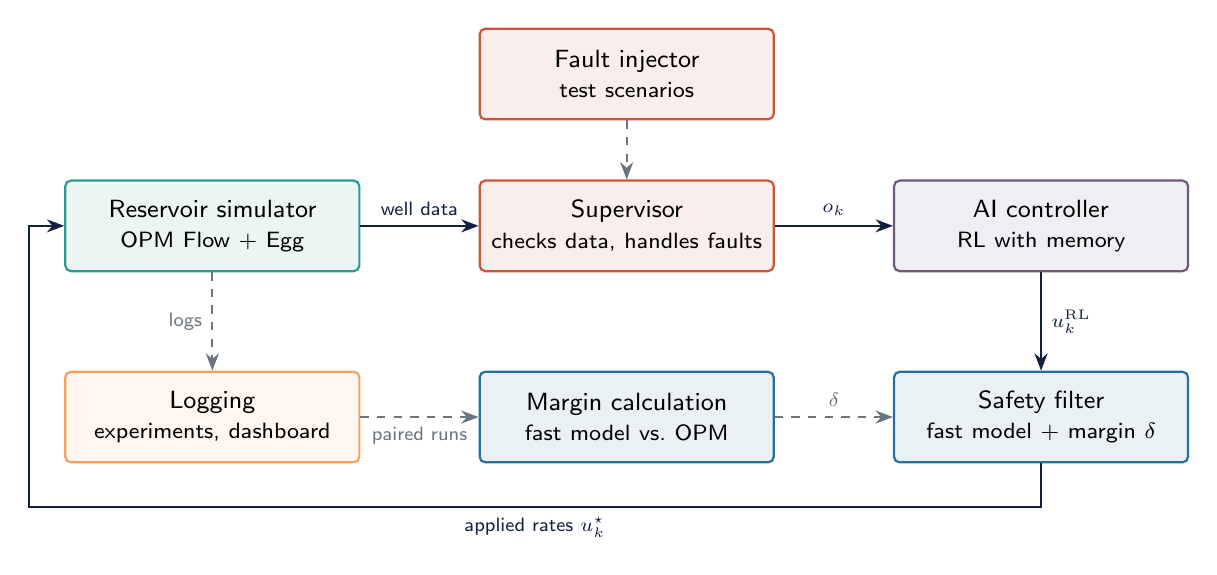
\begin{tikzpicture}[font=\sffamily\small,
  box/.style={draw=#1,fill=#1!10,rounded corners=2pt,line width=0.8pt,
    minimum height=1.15cm,text width=3.5cm,align=center},
  arr/.style={-{Stealth[length=2.2mm]},line width=0.8pt,aurNavy},
  off/.style={-{Stealth[length=2.2mm]},line width=0.8pt,aurGrey,dashed}]
\node[box=cAziz] (res) {Reservoir simulator\\\footnotesize OPM Flow + Egg};
\node[box=cTimur,right=1.5cm of res] (sup) {Supervisor\\\footnotesize checks data, handles faults};
\node[box=cAbdu,right=1.5cm of sup] (ctl) {AI controller\\\footnotesize RL with memory};
\node[box=cIsmael,below=1.25cm of ctl] (filt) {Safety filter\\\footnotesize fast model + margin $\delta$};
\node[box=cIsmael,below=1.25cm of sup] (cal) {Margin calculation\\\footnotesize fast model vs.\ OPM};
\node[box=cTimur,above=0.75cm of sup] (fault) {Fault injector\\\footnotesize test scenarios};
\node[box=cMahdi,below=1.25cm of res] (tel) {Logging\\\footnotesize experiments, dashboard};
\draw[arr] (res) -- node[above,font=\sffamily\scriptsize]{well data} (sup);
\draw[arr] (sup) -- node[above,font=\sffamily\scriptsize]{$o_k$} (ctl);
\draw[arr] (ctl) -- node[right,font=\sffamily\scriptsize]{$u^{\mathrm{RL}}_k$} (filt);
\draw[arr] (filt.south) -- ++(0,-0.55) -| node[pos=0.25,below,font=\sffamily\scriptsize]{applied rates $u^\star_k$} ($(res.south west)+(-0.45,-0.0)$) |- (res.west);
\draw[off] (cal) -- node[above,font=\sffamily\scriptsize]{$\delta$} (filt);
\draw[off] (fault) -- (sup);
\draw[off] (res) -- node[left,font=\sffamily\scriptsize]{logs} (tel);
\draw[off] (tel) -- node[below,font=\sffamily\scriptsize]{paired runs} (cal);
\end{tikzpicture}
\caption{The \aur{} control loop (solid arrows) and the supporting parts (dashed arrows).
Colours show who owns each part: Aziz (teal), Timur (red), Abdurrahman (purple), Ismael
(blue), Mahdi (orange).}\label{fig:arch}
\end{figure}

The controller's limited view is enforced in the code, not just by agreement. The
underground pressures and the detailed simulator's result go only to logging, margin
calculation and final testing. An automated test fails if any of that data shows up in what
the controller sees. Everything is written in Python and runs on team laptops or one
workstation. OPM Flow runs in a Docker container with a fixed version, so every member uses
exactly the same simulator. The parts exchange data in agreed formats, so members can build
and test their own part before the others are finished.

\subsection{Reservoir simulation (\AzizS)}

The Egg input files are prepared by a script from the published download and are never
edited by hand. A reservoir version is chosen by swapping in its rock-property file. The
controller has to change the injection rates at every decision and then continue the same
simulation. Our default way to do this is to run OPM up to step $k$, save its state, and
restart from that state with the new rates for step $k+1$. OPM also has a Python interface
that may be faster. Timing both options is the first implementation task. Every step is
checked: the simulator finished without error, the expected output exists, the requested
rates were applied, and the results make physical sense (no negative flows, water cut
between 0 and 1, totals that add up). To measure the fast model's error, the same saved
state can be re-run with different candidate decisions, which gives the detailed
simulator's answer for exactly the situation the fast model was asked about.

\subsection{AI controller (\AbduS)}

The simulation is wrapped in the standard Gymnasium interface. \Cref{tab:obs} summarizes
what the controller sees and does. It is deliberately not given the underground pressures,
the rock properties, or which reservoir version it is running on. That is what gives it
only a limited view.

\begin{table}[!htbp]
\caption{Proposed observations, actions and score for the AI controller.}\label{tab:obs}
\small
\begin{tabularx}{\textwidth}{@{}P{2.4cm}L@{}}
\toprule
\textbf{Observation} & For each producer: oil rate, water rate, water cut, BHP. For each injector: the rate actually applied, BHP. Overall: fraction of time elapsed, the previous decision, and, from the supervisor, whether each value is valid and how old it is. \\
\textbf{Action} & 8 injection rates, one per injector, each within the range the Egg model allows (up to \SI{79.5}{\cubic\metre\per\day}). \\
\textbf{Decision interval} & \emph{Proposed:} every 90 days, which gives 40 decisions over the reservoir's 3,600-day life. Chosen from 30, 60 and 90 days; shorter intervals give more control but cost more computing. \\
\textbf{Score (reward)} & Money earned in each step: oil revenue minus the cost of handling produced water and of injecting water. The prices are written down as an explicit assumption, and we test how sensitive the results are to them. \\
\textbf{One run} & One full reservoir life on one reservoir version from the development set. \\
\bottomrule
\end{tabularx}
\end{table}

Training directly in OPM may be too slow, because RL needs many simulated lifetimes. So
most training is done in a fast stand-in simulation built from the fast model, and the
controller is then refined and always tested in OPM. The versions with and without memory
are trained under the same conditions, each with at least five different random seeds
\cite{henderson2018matters}. Two simple controllers serve as baselines: the fixed injection
rates that come with Egg, and a hand-written rule that sends less water to injectors whose
nearby producers are producing more and more water.

\subsection{Fast model and safety filter (\IsmaelS)}

In the form of CRM we use, each injector--producer pair has its own connection. The liquid
that injector $i$ contributes to producer $j$ over a time step $\Delta t$ is
\begin{equation}\label{eq:crm}
q_{ij}(t_k) = q_{ij}(t_{k-1})\,e^{-\Delta t/\tau_{ij}}
  + \bigl(1-e^{-\Delta t/\tau_{ij}}\bigr) f_{ij}\, I_i(t_k),
\end{equation}
where $I_i$ is the injection rate, $f_{ij}$ (between 0 and 1) is the share of injector
$i$'s water that reaches producer $j$, and $\tau_{ij}$ sets how quickly the producer
responds. These values are fitted to OPM runs in which the injection rates are varied. The
data used for fitting are never reused to judge how good the fit is.

The limit we protect is the bottom-hole pressure of each injector, which must stay below
$y_{\max}=\SI{420}{\bar}$. This is the limit set in the Egg model. We use it as the rule
for our experiment; we do not claim it is the pressure at which real rock would crack. CRM
predicts flow rates, not pressure, so we add a simple straight-line relation between each
injector's rate and its pressure, fitted to OPM data and updated at each step with the
latest measured pressure. The predicted pressure is then a straight-line function of the
decision $u$: $\hat y_{k+1}(u)=c_k+G_k u$. Finding the closest safe decision becomes a
small optimization problem:
\begin{equation}\label{eq:qp}
u^\star_k = \arg\min_{u,\;s\ge 0}\;
 (u-u^{\mathrm{RL}}_k)^{\!\top} W (u-u^{\mathrm{RL}}_k) + \rho\,\mathbf{1}^{\!\top}s
\quad\text{s.t.}\quad
 c_k + G_k u + \delta \le y_{\max} + s,\quad u_{\min}\le u\le u_{\max}.
\end{equation}
In words: stay as close as possible to what the controller proposed, while keeping the
predicted pressure plus the margin $\delta$ under the limit, and the rates within their
allowed range. The extra variable $s$ lets the solver return an answer even when no fully
safe decision exists. It is penalized heavily, and any use of it is logged as a failure of
the filter. With $\delta=0$ the filter trusts the fast model completely; we call this the
\emph{plain} filter. The problem is solved with OSQP \cite{stellato2020osqp}.

Two details matter. First, the Egg input files tell the simulator itself to cap injector
pressure at \SI{420}{\bar} by quietly pumping less water than requested. With that cap in
place OPM would never report a pressure above the limit, and we could not see violations.
For testing we raise the simulator's cap, so that OPM reports the pressure the requested
rate really needs. Second, if injector pressure never gets close to the limit, there is
nothing for the filter to do and the comparison tells us nothing. We check this early. If
it is the case, we switch to a limit on produced water, which the fast model can also
predict (\cref{sec:risks}).

\Cref{fig:margin-concept} illustrates the idea behind the margin, which the next subsection
explains.

\begin{figure}[!htbp]
\centering
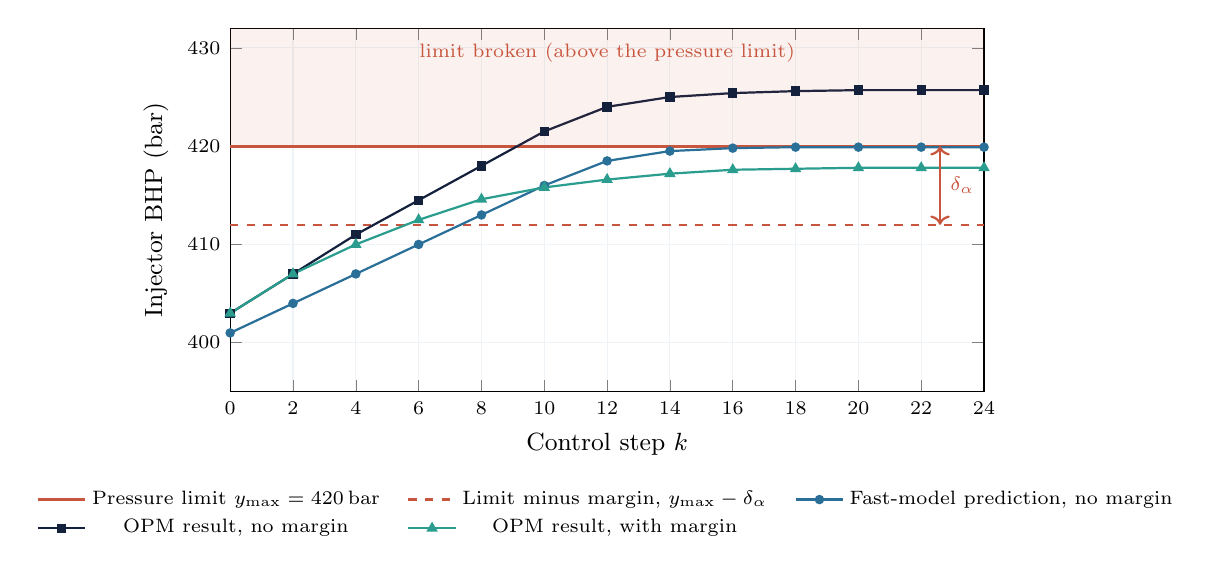
\begin{tikzpicture}
\begin{axis}[width=0.92\textwidth,height=6.2cm,
  xlabel={Control step $k$},ylabel={Injector BHP (\si{\bar})},
  xmin=0,xmax=24,ymin=395,ymax=432,
  legend style={at={(0.5,-0.24)},anchor=north,font=\scriptsize,draw=none,legend columns=3,/tikz/every even column/.append style={column sep=8pt}},
  tick label style={font=\scriptsize},label style={font=\small},
  grid=major,grid style={aurLight}]
  \addplot[aurRed,very thick,domain=0:24] {420};
  \addlegendentry{Pressure limit $y_{\max}=\SI{420}{\bar}$}
  \addplot[aurRed,dashed,thick,domain=0:24] {412};
  \addlegendentry{Limit minus margin, $y_{\max}-\delta_\alpha$}
  \addplot[aurBlue,thick,mark=*,mark size=1.3pt] coordinates
    {(0,401)(2,404)(4,407)(6,410)(8,413)(10,416)(12,418.5)(14,419.5)(16,419.8)(18,419.9)(20,419.9)(22,419.9)(24,419.9)};
  \addlegendentry{Fast-model prediction, no margin}
  \addplot[aurNavy,thick,mark=square*,mark size=1.3pt] coordinates
    {(0,403)(2,407)(4,411)(6,414.5)(8,418)(10,421.5)(12,424)(14,425)(16,425.4)(18,425.6)(20,425.7)(22,425.7)(24,425.7)};
  \addlegendentry{OPM result, no margin}
  \addplot[aurTeal,thick,mark=triangle*,mark size=1.6pt] coordinates
    {(0,403)(2,407)(4,410)(6,412.5)(8,414.6)(10,415.8)(12,416.6)(14,417.2)(16,417.6)(18,417.7)(20,417.8)(22,417.8)(24,417.8)};
  \addlegendentry{OPM result, with margin}
  \draw[<->,aurRed,thick] (axis cs:22.6,412) -- (axis cs:22.6,420) node[midway,right,font=\scriptsize] {$\delta_\alpha$};
  \fill[aurRed,opacity=0.08] (axis cs:0,420) rectangle (axis cs:24,432);
  \node[font=\scriptsize,text=aurRed,anchor=north] at (axis cs:12,431.5) {limit broken (above the pressure limit)};
\end{axis}
\end{tikzpicture}
\caption[Conceptual illustration of the \aur{} mechanism]{Illustration of the idea (not experimental data). A filter with no margin keeps
the \emph{predicted} pressure below the limit, but the fast model predicts too low, so the
pressure in the detailed simulator goes above it. Adding the measured margin
$\delta_\alpha$ keeps the actual pressure below the limit while staying close to it.}
\label{fig:margin-concept}
\end{figure}

\subsection{Measuring the fast model's error (\IsmaelS{} with \AzizS)}

For the same situation and the same decision, let $y^{\mathrm{OPM}}_{k+1}$ be the pressure
from the detailed simulator and $\hat y^{\mathrm{ROM}}_{k+1}$ the fast model's prediction.
The error is
\begin{equation}\label{eq:res}
r_{k+1} = y^{\mathrm{OPM}}_{k+1} - \hat y^{\mathrm{ROM}}_{k+1}.
\end{equation}
A positive error is the dangerous kind: the fast model predicted too low, so the filter
thinks an unsafe decision is safe. We collect $n$ such errors on the reservoir versions set
aside for this, sort them from smallest to largest, and take the value below which a chosen
share of them fall. With a target of 95\% (that is, $\alpha=0.05$):
\begin{equation}\label{eq:margin}
\delta_\alpha = r_{(\lceil (n+1)(1-\alpha)\rceil)} .
\end{equation}
This is the one-sided conformal bound described in the background
\cite{lei2018conformal}. In theory the fast model's error on a new case is then below
$\delta_\alpha$ at least 95\% of the time, provided the new cases resemble the measured
ones. Reservoir data only partly meet that condition, because errors close together in time
or at neighbouring wells are related. So we treat 95\% as a target and report what is
actually achieved. To estimate how well the margin carries over to a new reservoir version,
we repeatedly leave one version out, compute the margin from the rest, and check it on the
one left out. We also compute a separate margin for each injector. If the margin does not
carry over, the fallback is a version that adjusts itself over time \cite{gibbs2021aci}.
The planned amount of data is 20 reservoir versions $\times$ 20 points in time $\times$ 5
candidate decisions, about 2,000 short OPM runs.

\subsection{Fault testing and failure handling (\TimurS)}

A control system that has only been tested with perfect data has not really been tested.
This part has two pieces: a \emph{fault injector} that creates realistic problems on
demand, and a \emph{supervisor} that detects them while the system runs and keeps it in a
defined safe mode. The fault scenarios are based on evidence, not invented: our review of
real field data (\cref{sec:data}) shows missing pressure readings, wells that change role
and impossible negative volumes. \Cref{tab:faults} lists the kinds of fault.

\begin{table}[!htbp]
\caption{Kinds of fault, what each is based on, and the expected response.}\label{tab:faults}
\small
\begin{tabularx}{\textwidth}{@{}P{2.3cm}P{4.2cm}LP{3.3cm}@{}}
\toprule
\textbf{Kind of fault} & \textbf{Examples} & \textbf{Based on} & \textbf{Response} \\
\midrule
Missing data & sensor drops out; gaps that come and go & missing pressure in Volve & keep the last good value for a limited time; degraded mode \\
Frozen or delayed data & value stops changing; old measurement arrives late & common failures of measurement systems & check how recent the data are; degraded mode \\
Invalid data & not a number, negative rate, water cut above 1 & Volve records with negative volumes & reject the value; degraded mode \\
Noise and spikes & random noise, outliers & measurement noise & smooth the input; log \\
Model drift & fast-model values shifted; unfamiliar reservoir & known CRM error \cite{mamghaderi2021crm} & larger margin, or fallback \\
Controller fault & invalid or out-of-range decision; no answer in time & software failure & reject; fallback \\
Filter fault & no safe decision found, or solver too slow & optimization failure & fallback \\
Simulator fault & OPM step fails or takes too long & numerical failure & mark the run invalid; keep it \\
\bottomrule
\end{tabularx}
\end{table}

The supervisor is a small state machine that always behaves the same way for the same
inputs (\cref{fig:supervisor}). It checks every measurement (right format, sensible range,
a real number, recent enough) and uses timers to detect parts that stop responding. In
\emph{Degraded} mode the controller is given the last good values, as long as they are not
too old, and the filter may use a larger margin. In \emph{Fallback} mode a cautious action
is applied: the last decision known to be safe, reduced by a documented factor. \emph{Safe
hold} ends the run and flags it. The supervisor waits for conditions to stay good for
several steps before switching back, so it does not flip rapidly between modes.

\begin{figure}[!htbp]
\centering
\begin{adjustbox}{max width=\textwidth}
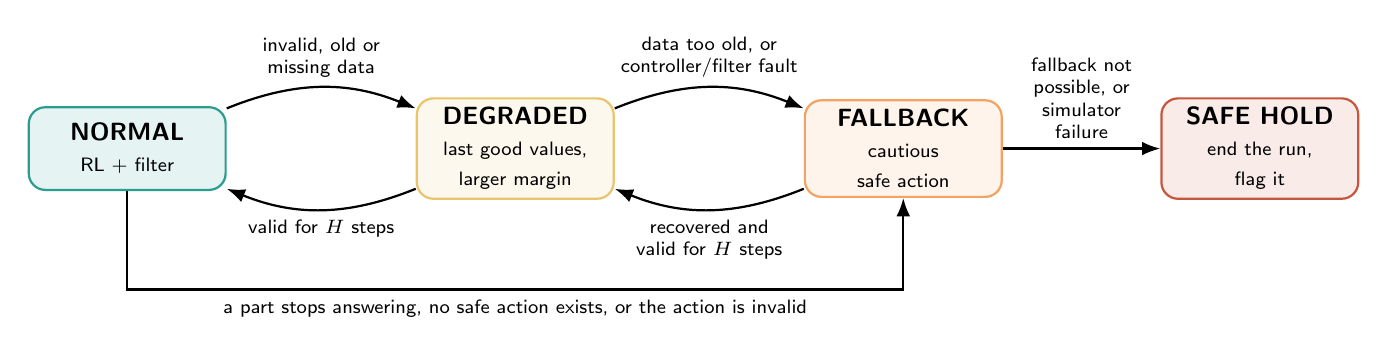
\begin{tikzpicture}[font=\sffamily\small,>=Latex,node distance=2.4cm,
  st/.style={draw=#1,fill=#1!12,thick,rounded corners=6pt,minimum width=2.5cm,minimum height=1.05cm,align=center},
  tr/.style={font=\sffamily\scriptsize,align=center}]
  \node[st=aurTeal] (n) {\textbf{NORMAL}\\{\scriptsize RL + filter}};
  \node[st=aurSand,right=of n] (d) {\textbf{DEGRADED}\\{\scriptsize last good values,}\\{\scriptsize larger margin}};
  \node[st=aurOrange,right=of d] (f) {\textbf{FALLBACK}\\{\scriptsize cautious}\\{\scriptsize safe action}};
  \node[st=aurRed,right=2.0cm of f] (h) {\textbf{SAFE HOLD}\\{\scriptsize end the run,}\\{\scriptsize flag it}};
  \draw[->,thick] (n) to[bend left=22] node[above,tr]{invalid, old or\\missing data} (d);
  \draw[->,thick] (d) to[bend left=22] node[below,tr]{valid for $H$ steps} (n);
  \draw[->,thick] (d) to[bend left=22] node[above,tr]{data too old, or\\controller/filter fault} (f);
  \draw[->,thick] (f) to[bend left=22] node[below,tr]{recovered and\\valid for $H$ steps} (d);
  \draw[->,thick] (f) -- node[above,tr]{fallback not\\possible, or\\simulator\\failure} (h);
  \draw[->,thick] (n.south) -- ++(0,-1.25) -| node[pos=0.25,below,tr]{a part stops answering, no safe action exists, or the action is invalid} (f.south);
\end{tikzpicture}
\end{adjustbox}
\caption[Runtime supervisor state machine]{The supervisor's state machine. Every change of mode is logged with its cause, and
the time to detect a fault is measured from the moment the fault injector started it.}
\label{fig:supervisor}
\end{figure}

Each scenario is an automated test with an expected sequence of modes. We report how often
faults are detected, how quickly, how many false alarms occur on clean runs, and how much
performance is lost.

\subsection{Logging, experiments and dashboard (\MahdiS)}

One log record is written per decision step, with each stage stored separately: the
measurements, the proposed decision, the fast model's prediction, the margin, the applied
decision, what the simulator did, the result, the supervisor's mode and timings. Every run
also saves a record of exactly how it was produced: the version of the code, the settings,
which reservoir version, the random seeds, the simulator version and whether it succeeded.
A batch runner works through every combination of controller, reservoir version and seed in
parallel. It can resume after an interruption, and it keeps failed runs, with the reason,
instead of discarding them. The dashboard reads only these logs, so it shows what actually
happened.

% We have to over this as a group, especially cuz its asking for a general alternative to the whole system
% \subsection{Alternatives considered}

% For the system as a whole we compared five designs (\cref{tab:altsys}). Designs C and D
% are the same system as ours with the margin set to zero or to a guessed constant, so
% comparing C, D and E is a fair test in which only one thing changes. For each main
% component we then scored the options against weighted criteria: whether the research
% result will be valid, whether it can be done in two terms, and whether it can be
% reproduced. The scoring tables are in the repository and \cref{tab:alt} gives the outcome.

% \begin{table}[!htbp]
% \caption{System designs considered.}\label{tab:altsys}
% \small
% \begin{tabularx}{\textwidth}{@{}P{3.6cm}LLP{1.9cm}@{}}
% \toprule
% \textbf{Design} & \textbf{Strengths} & \textbf{Weaknesses for our question} & \textbf{Decision} \\
% \midrule
% A. Classical model-based control using the CRM, no learning & Well established; handles limits directly & Suffers from the same fast-model error; does not test learned control & Not built \\
% B. RL trained to respect the limits by itself & A single component; strong recent results \cite{chen2025wcsac,achiam2017cpo} & Limits hold only on average; model error is hidden inside the controller & Optional comparison \\
% C. RL + filter that trusts the fast model & Checks every decision & Safe only as far as the fast model is right & Baseline (plain filter) \\
% D. RL + filter with a fixed cautious margin & Simple; reduces violations & Margin is a guess; may give up production for nothing & Baseline (fixed margin) \\
% \textbf{E. \aur{}: RL + filter with a measured margin} & Checks every decision; margin based on error measured on separate reservoirs & More parts; depends on the margin carrying over to new reservoirs & \textbf{Selected} \\
% \bottomrule
% \end{tabularx}
% \end{table}

% \begin{table}[!htbp]
% \caption{Design choices.}\label{tab:alt}
% \small
% \begin{tabularx}{\textwidth}{@{}P{2.3cm}P{2.6cm}P{3.1cm}L@{}}
% \toprule
% \textbf{Decision} & \textbf{Chosen} & \textbf{Alternatives} & \textbf{Main reason}\\
% \midrule
% Simulator & OPM Flow & MRST, commercial simulators & Free, runs Egg as published, and the team has already run it\\
% Test reservoir & Egg (100 versions) & SPE10, OLYMPUS, a model of Volve & Many versions allow separate ones for training, margin and final test; each run is quick\\
% Fast model & CRM, one connection per injector--producer pair & Simpler CRM, neural-network model & Its parameters have a physical meaning, and it keeps the safety filter a simple optimization problem\\
% Controller & PPO with memory & PPO fed its last few observations, SAC & Learns for itself what to remember; the simpler option is the fallback\\
% Safety method & Filter that corrects each decision & Penalty in the score, limits learned in training & Checks every decision, shows why it changed one, and has one clear place to add the margin\\
% Margin & Percentile of measured errors (conformal) & Assume bell-curve errors; use the worst error seen & Makes no assumption about how the errors are distributed\\
% \bottomrule
% \end{tabularx}
% \end{table}

% There's a lot of fake claims, made up data, and false info here
% % ============================================================== 5
% \section{Data, Simulation and Feasibility}\label{sec:data}

% \aur{} uses three outside resources, each for a different purpose (\cref{tab:res}).

% \begin{table}[!htbp]
% \caption{Outside resources, what each is for, and what each cannot tell us.}\label{tab:res}
% \small
% \begin{tabularx}{\textwidth}{@{}P{2.2cm}P{3.6cm}LP{3.2cm}@{}}
% \toprule
% \textbf{Resource} & \textbf{What it is} & \textbf{What it lets us do} & \textbf{What it cannot show}\\
% \midrule
% Egg model \cite{jansen2014egg} & A published made-up reservoir in 100 versions & Run repeatable experiments on many different reservoirs & That results hold on a real field\\
% OPM Flow \cite{rasmussen2021opm} & A detailed open-source simulator & See the result of any decision, including ones nobody ever made & What a real reservoir would do\\
% Volve \cite{equinor2018volve} & Recorded data from a real oil field & See what real measurements and real data problems look like & How a different controller would have done\\
% \bottomrule
% \end{tabularx}
% \end{table}

% \textbf{We generate our experimental data ourselves.} Every OPM run produces a complete
% record of flow rates and pressures for every well at every step. The error measurements,
% the margin and the final test results all come from our own simulations. What limits us is
% computing time, not the amount of data available.

% \textbf{Egg.} We downloaded the model from its permanent online record
% \cite{egg2014dataset} and checked it in detail. All 100 versions load correctly. Injectors
% pump \SI{79.5}{\cubic\metre\per\day} each with a \SI{420}{\bar} pressure limit, producers
% are held at \SI{395}{\bar}, and the simulation covers 120 steps of 30 days. Egg is
% deliberately small and simple. That is what makes thousands of runs affordable, and we do
% not present it as a real reservoir. \Cref{tab:egg} lists its main properties and
% \cref{fig:egg-wells} shows where the wells are.

% \noindent \begin{minipage}[t]{0.52\textwidth}
% \vspace{0pt}
% \captionof{table}[Audited properties of the Egg case used by \aur]{Properties of the Egg model, as we checked them.}
% \label{tab:egg}
% \small
% \begin{tabularx}{\linewidth}{@{}P{3.1cm}L@{}}
% \toprule
% Grid & $60\times60\times7$ = 25{,}200 cells; 18{,}553 active \\
% Cell size & \SI{8}{\metre}$\times$\SI{8}{\metre}$\times$\SI{4}{\metre} \\
% Porosity; net-to-gross & 0.2 (same everywhere); 1 \\
% Fluids & oil and water (metric units) \\
% Geology & 100 versions of the rock properties (all read correctly) + one base version \\
% Wells & 8 water injectors, 4 producers, open to all 7 layers \\
% Injector setting & rate \SI{79.5}{\cubic\metre\per\day}, BHP limit \SI{420}{\bar} \\
% Producer setting & BHP held at \SI{395}{\bar} \\
% Schedule & 120 steps $\times$ \SI{30}{\day} = \SI{3600}{\day} \\
% Outputs & field and well rates and totals; pressure and water content of every cell (in the saved state) \\
% \bottomrule
% \end{tabularx}
% \end{minipage}\hfill
% \begin{minipage}[t]{0.44\textwidth}
% \vspace{0pt}
% \centering
% \begin{tikzpicture}
% \begin{axis}[width=6.9cm,height=6.9cm,xmin=-2,xmax=63,ymin=-2,ymax=63,clip=false,
%   xlabel={grid $I$},ylabel={grid $J$},axis equal image,
%   tick label style={font=\scriptsize},label style={font=\scriptsize},
%   xtick={0,20,40,60},ytick={0,20,40,60},
%   axis background/.style={fill=aurSand!18}]
%   \addplot[only marks,mark=triangle*,mark size=3.2pt,color=aurBlue,
%     nodes near coords,point meta=explicit symbolic,
%     every node near coord/.style={font=\scriptsize\sffamily\bfseries,color=aurBlue,anchor=west,xshift=1pt}]
%     coordinates {(5,57)[I1] (30,53)[I2] (2,35)[I3] (27,29)[I4] (50,35)[I5] (8,9)[I6] (32,2)[I7] (57,6)[I8]};
%   \addplot[only marks,mark=*,mark size=3pt,color=black!80,
%     nodes near coords,point meta=explicit symbolic,
%     every node near coord/.style={font=\scriptsize\sffamily\bfseries,color=black,anchor=west,xshift=1pt}]
%     coordinates {(16,43)[P1] (35,40)[P2] (23,16)[P3] (43,18)[P4]};
% \end{axis}
% \end{tikzpicture}
% \captionof{figure}[Egg well locations]{Egg well locations (from the input files we checked): injectors
% \textcolor{aurBlue}{$\blacktriangle$}, producers $\bullet$.}
% \label{fig:egg-wells}
% \end{minipage}
% \vspace{0.6em}

% \textbf{Running the detailed simulator.} The step the whole project depends on already
% works. OPM Flow ran the Egg model from start to finish and produced output our software can
% read. We then changed one setting, lowering injector 1 from 79.5 to
% \SI{60}{\cubic\metre\per\day}, and ran it again. OPM applied exactly that change (total
% injection went from 636.0 to \SI{616.5}{\cubic\metre\per\day}), and production responded
% (\cref{fig:f3}): total oil changed by $-0.35\%$ and total produced water by $-3.82\%$. This
% does not mean 60 is a better setting. It shows that our software can change a decision in
% the detailed simulator and measure what happens, which is what a controller needs.

% \begin{figure}[!htbp]
% \centering
% \begin{tikzpicture}
% \begin{axis}[width=0.86\textwidth,height=5.0cm,
%   xlabel={Simulated time (days)},ylabel={Field rate (m$^3$/d)},
%   xmin=0,xmax=3600,ymin=0,ymax=700,xtick={0,600,...,3600},
%   grid=major,grid style={aurLight},
%   legend style={font=\footnotesize,at={(0.5,1.03)},anchor=south,legend columns=4,draw=none},
%   every axis plot/.append style={line width=1pt}]
% \addplot[aurNavy] table[x=day,y=FOPRb]{\FthreeData};
% \addplot[aurNavy,dashed] table[x=day,y=FOPRp]{\FthreeData};
% \addplot[aurTeal] table[x=day,y=FWPRb]{\FthreeData};
% \addplot[aurTeal,dashed] table[x=day,y=FWPRp]{\FthreeData};
% \legend{Oil, original,Oil, changed,Water, original,Water, changed}
% \end{axis}
% \end{tikzpicture}
% \caption{Total oil and water production from OPM Flow for the original Egg settings and
% with injector 1 lowered from 79.5 to \SI{60}{\cubic\metre\per\day} (the team's own test
% run).}\label{fig:f3}
% \end{figure}

% \textbf{Volve.} The oil company Equinor released recorded data from its Volve field in the
% North Sea for research and teaching \cite{equinor2018volve}. Our review found seven wells
% (two water injectors and five producers) and about 15,600 daily records. The data are
% messy: downhole pressure is missing in about 43\% of records, the injectors have almost no
% pressure data, some wells switch between injecting and producing, and a few records contain
% impossible negative volumes. As a first test, we fitted the CRM to monthly Volve data and
% checked its forecasts on the last 30\% of each producer's history. It beat the simplest
% possible forecast (``next month equals this month'') for only one of the five producers. We
% draw two lessons. Real field data are much messier than simulator output, which is what our
% fault scenarios are based on. And a simple model's error on real data is large, so it has
% to be measured, not assumed small. We use Volve only for these two purposes. A recording of
% the past cannot show what would have happened under different decisions.

% \textbf{Feasibility.} Before committing to this design we turned each major doubt into a
% question we could test (\cref{tab:feas}). The results are saved in the repository. The
% remaining parts use well-maintained open-source libraries. The main open question is how
% fast OPM can be run one decision at a time, and that is the first thing we will measure.

% \begin{table}[!htbp]
% \caption{Feasibility checks completed.}\label{tab:feas}
% \small
% \begin{tabularx}{\textwidth}{@{}lP{4.4cm}LP{1.6cm}@{}}
% \toprule
% \textbf{ID} & \textbf{Question} & \textbf{Main evidence} & \textbf{Result} \\
% \midrule
% F1 & Do the data and tools exist, and can we get them? & Egg downloaded from its permanent record and checked; OPM manual and Volve licence saved & Pass \\
% F2 & Is the Egg dataset complete and usable? & Grid, wells, well settings and schedule all read correctly; all 100 versions valid & Pass \\
% F3 & Can OPM run Egg and respond to our changes? & Full 3,600-day run without error; a change to one injector applied exactly; producers responded & Pass \\
% F4 & Is there a source for every piece of data the design needs? & Every input and output in the design is available directly, can be calculated, or needs code we will write & Pass \\
% F5 & Can our assumptions about the reservoir be defended? & Each assumption checked against the Egg paper, the OPM manual and the CRM literature; none rejected & Pass with conditions \\
% F6 & Has this already been done? & Literature search aimed at finding the same work; our claim narrowed to what is new & Pass with conditions \\
% F7 & Does real field data support the approach? & Volve data reviewed; injection and production records exist; data problems listed & Pass \\
% \bottomrule
% \end{tabularx}
% \end{table}

% ============================================================== 6
\section{Evaluation: How We Will Know Whether It Worked}\label{sec:eval}

\subsection{Research question and hypotheses}

\begin{keybox}[title=Research question.]
If the safety filter includes a margin based on the fast model's measured error, does the
controller break the pressure limit less often on reservoir versions it has never seen,
compared with the same controller and a filter with no margin, and without losing much
oil production?
\end{keybox}

\begin{itemize}
\item[H1] \emph{The error matters.} The fast model predicts too low often enough that the plain filter still lets violations through in OPM.
\item[H2] \emph{Main hypothesis.} On unseen reservoir versions, the filter with the measured margin has fewer or smaller violations than the plain filter.
\item[H3] \emph{Cost.} For a similar number of violations, the measured margin gives up less oil (or money) than a fixed, guessed margin.
\item[H4] \emph{Memory.} Given the same measurements, the controller with memory does better than the one without.
\end{itemize}

\subsection{Experiment design}

This follows the usual machine-learning practice of separate training and test data, except
that we split reservoir versions instead of rows of a table. The 100 Egg versions are
divided once: 60 for development (training, tuning and demonstrations), 20 for measuring
the fast model's error, and 20 kept unseen for the final test. The assignment is random
with a fixed seed and is saved in the repository. The experiment software refuses to load
the test versions until the test plan has been fixed (\cref{fig:split}).

\begin{figure}[!htbp]
\centering
\begin{tikzpicture}[font=\sffamily\small,>=Latex]
  \foreach \i in {0,...,59}{\fill[aurBlue!70] ({mod(\i,20)*0.33},{-floor(\i/20)*0.33}) rectangle ++(0.28,0.28);}
  \foreach \i in {0,...,19}{\fill[aurOrange!85] ({7.2+mod(\i,10)*0.33},{-floor(\i/10)*0.33}) rectangle ++(0.28,0.28);}
  \foreach \i in {0,...,19}{\fill[aurRed!80] ({11.0+mod(\i,10)*0.33},{-floor(\i/10)*0.33}) rectangle ++(0.28,0.28);}
  \node[anchor=south west,font=\sffamily\small\bfseries,text=aurBlue] at (0,0.35) {Development (60)};
  \node[anchor=south west,font=\sffamily\small\bfseries,text=aurOrange!80!black] at (7.2,0.35) {Calibration (20)};
  \node[anchor=south west,font=\sffamily\small\bfseries,text=aurRed] at (11.0,0.35) {Unseen test (20)};
  \node[anchor=north west,align=left,font=\sffamily\scriptsize] at (0,-0.8) {training, fast-model design,\\tuning, debugging, demo};
  \node[anchor=north west,align=left,font=\sffamily\scriptsize] at (7.2,-0.5) {matching fast-model/OPM runs,\\errors $\rightarrow$ margin $\delta_\alpha$};
  \node[anchor=north west,align=left,font=\sffamily\scriptsize] at (11.0,-0.5) {locked until the test plan is\\fixed; final test only};
  \draw[aurRed,thick,dashed,rounded corners] (10.85,0.9) rectangle (14.4,-1.35);
  \node[font=\sffamily\scriptsize\bfseries,text=aurRed,anchor=north] at (12.62,-1.5) {\faLock\ fixed list, every access logged};
\end{tikzpicture}
\caption[Proposed geological partition of the 100 Egg permeability realizations]{Proposed split of the 100 Egg reservoir versions. No version moves between
groups once the split is fixed.}
\label{fig:split}
\end{figure}

The main experiment compares seven controllers, each adding one feature to the one before
(\cref{tab:ladder}). The comparisons that answer the research question are C4 against C6
and C5 against C6.

\begin{table}[!htbp]
\caption{The controllers compared on unseen reservoir versions.}\label{tab:ladder}
\small
\begin{tabularx}{\textwidth}{@{}lP{5.6cm}Ll@{}}
\toprule
\textbf{ID} & \textbf{Controller} & \textbf{What it tells us} & \textbf{Hyp.}\\
\midrule
C0 & Fixed rates that come with Egg & The baseline: no control at all & --\\
C1 & Hand-written rule & Does learning beat a simple rule? & --\\
C2 & RL without memory, no filter & How well learning does without memory & H4\\
C3 & RL with memory, no filter & Whether memory helps & H4\\
C4 & RL with memory + plain filter (no margin) & Does trusting the fast model still allow violations? & H1\\
C5 & RL with memory + fixed margin (several sizes) & What a guessed margin costs in production & H3\\
C6 & RL with memory + measured margin & Does a margin based on measured error help? & H2, H3\\
\bottomrule
\end{tabularx}
\end{table}

Everything we report is measured from what happened in the detailed simulator, never from
the fast model's predictions (\cref{tab:metrics}).

\begin{table}[!htbp]
\caption{What we measure.}\label{tab:metrics}
\small
\begin{tabularx}{\textwidth}{@{}P{2.9cm}L@{}}
\toprule
\textbf{Group} & \textbf{Measurements} \\
\midrule
Production and money & Total oil, total water produced and injected; the money-based score, and how much it changes with the assumed prices \\
Safety & How often the limit is broken; the largest and the total amount above the limit; how long violations last \\
Filter behaviour & How often the filter changes a decision and by how much; how often no safe decision exists \\
Fast-model accuracy & The spread of its errors; average error size; how bad the worst under-predictions are; by reservoir version and well \\
Margin & How often the margin actually covers the error, compared with the 95\% target, on margin and on unseen reservoirs \\
Failure handling & How often and how quickly faults are detected; false alarms; performance lost under faults \\
Computing time & Time per decision for the controller, fast model and filter; OPM time per step \\
\bottomrule
\end{tabularx}
\end{table}

\textbf{Test plan and statistics.} Before the final test we fix everything that could
affect the result and save it as a tagged version of the repository: the split of reservoir
versions, what the controller sees and controls, the prices in its score, the 95\% target,
what we measure, the fixed margin sizes, the number of seeds and the statistical method.
The 20 test versions are then used once. Each learned controller is trained with at least
five random seeds, and each is tested on all 20 test versions. Because every controller is
tested on the same versions, we compare them version by version. We report 95\% confidence
intervals computed by bootstrap resampling \cite{agarwal2021precipice}, and we only claim a
difference when the interval does not include zero. The final test is about 840 full
simulations. If one takes $T$ minutes, the total is about $14T$ hours of computing, which
is why measuring $T$ comes first.

\subsection{Testing}

Each design level has a matching test level (the V-model), and every requirement in
\cref{sec:req} states how it is checked. \Cref{tab:tests} lists the levels. Automated
tests run on every proposed code change. They show that our written checks pass; whether
the results make physical sense is covered in the next subsection.

\begin{table}[!htbp]
\caption{Test levels.}\label{tab:tests}
\small
\begin{tabularx}{\textwidth}{@{}P{2.6cm}LP{2.9cm}@{}}
\toprule
\textbf{Level} & \textbf{Examples} & \textbf{When it runs} \\
\midrule
Unit and random-case & The filter changes decisions as little as possible and reports when no safe decision exists; the margin is the right percentile; CRM fitting recovers known values from generated data; supervisor mode changes & Every code change \\
Interface & Each data format exchanged between two parts is checked, using stand-ins for the part that produces it and the part that uses it & Every code change \\
Integration & Simulation wrapper with OPM for one step; controller with filter; logs are complete & Nightly or on request \\
System & A full simulation on a development reservoir reproduces a stored reference result & Before each milestone \\
Fault tests & Every fault scenario gives its expected sequence of modes and never an invalid decision & Before each milestone \\
Final test & All controllers compared on the unseen reservoirs under the fixed test plan & Once (M6) \\
\bottomrule
\end{tabularx}
\end{table}

\subsection{Telling right results from wrong ones}

No one on the team is a reservoir engineer, and we cannot ask an expert to review our system. So we check correctness at four levels:
\begin{itemize}
\item \emph{Does each part work?} Every component is tested on a case where we already know the answer. If we generate data from a CRM with known settings, fitting must recover those settings. If a decision is already safe, the filter must return it unchanged. On made-up errors with a known distribution, the margin must cover 95\% of them.
\item \emph{Did the experiment run as planned?} Saved run records and the guard on the test versions show that the experiment ran as specified. We also check results that can be predicted in advance: a margin of zero must behave exactly like the plain filter, and a bigger margin must never cause more violations.
\item \emph{Do the results make physical sense?} Basic rules are checked at every step, and we check that changes go in the right direction (pumping less water must not raise the pressure at that well). Our run of the original Egg settings is compared with the reference results published with Egg.
\end{itemize}

We write down what each possible result would mean before we see the results
(\cref{tab:interp}). Finding that the margin does not help is an acceptable outcome, and we
would report it along with the reason.

\begin{table}[!htbp]
\caption{What each possible result would mean, decided in advance.}\label{tab:interp}
\small
\begin{tabularx}{\textwidth}{@{}P{6.2cm}L@{}}
\toprule
\textbf{If we see\ldots} & \textbf{It means\ldots}\\
\midrule
C6 has fewer violations than C4, and more oil than C5 for similar violations & H2 and H3 are supported, for the conditions we tested\\
C6 and C4 about the same, both with almost no violations & The limit is rarely reached, or the fast model is good enough; H1 is not supported; try the produced-water limit\\
C6 and C4 about the same, both with violations & The margin is too small, or it did not carry over to new reservoir versions\\
C6 is safe but no better than C5 & A measured margin has no advantage over a guessed one here; H3 is rejected\\
C3 and C2 about the same & Memory does not help with these measurements; H4 is rejected\\
\bottomrule
\end{tabularx}
\end{table}

\subsection{Demonstration}

The supervisors were clear that a demonstration must not be numbers scrolling in a
terminal. The system is shown through an interactive dashboard 
% Timur has to decide what he's gonna do and fix this depending on that

\begin{figure}[!htbp]
\centering
\begin{adjustbox}{max width=\textwidth}
\begin{tikzpicture}[font=\sffamily\scriptsize,
  pane/.style={draw=aurGrey,fill=white,rounded corners=2pt,thick},
  ttl/.style={anchor=north west,font=\sffamily\scriptsize\bfseries,text=aurNavy}]
  \fill[aurLight,rounded corners=4pt] (-0.2,-0.2) rectangle (16.2,9.4);
  \fill[aurNavy,rounded corners=3pt] (0,8.7) rectangle (16,9.25);
  \node[text=white,anchor=west,font=\sffamily\small\bfseries] at (0.2,8.97) {AURORA};
  \node[text=white,anchor=west] at (1.9,8.97) {Run: C6 \textbullet{} reservoir dev-017 \textbullet{} seed 3 \qquad step 23 / 40 \quad day 2070};
  \node[text=white,anchor=east] at (15.8,8.97) {\faPlay\ \faPause\ \faStepForward\quad mode: \textcolor{aurTeal!60!white}{\textbf{NORMAL}}};
  % Panel 1: well map
  \draw[pane] (0,4.4) rectangle (5.2,8.5); \node[ttl] at (0.1,8.45) {1 \ Reservoir and wells};
  \shade[left color=aurBlue!45,right color=aurSand!60] (0.4,4.7) rectangle (4.8,7.9);
  \foreach \x/\y in {0.6/7.6,2.6/7.3,0.5/6.1,2.4/5.9,3.9/6.1,0.9/4.9,2.7/4.8,4.5/4.9}{\fill[aurBlue] (\x,\y) circle (0.1);}
  \foreach \x/\y in {1.5/6.8,3.0/6.6,2.0/5.3,3.4/5.4}{\fill[black] (\x,\y) circle (0.1);}
  \node[align=center,font=\sffamily\tiny] at (2.6,4.55) {water-content map; well markers sized by rate};
  % Panel 2: proposed vs applied
  \draw[pane] (5.4,4.4) rectangle (10.6,8.5); \node[ttl] at (5.5,8.45) {2 \ Controller vs.\ safety filter};
  \node[font=\sffamily\tiny,anchor=west] at (5.55,7.95) {\textcolor{aurPurple!70}{$\blacksquare$} proposed \quad \textcolor{aurBlue}{$\blacksquare$} applied};
  \foreach \i/\a/\b in {0/1.6/1.6,1/2.1/1.9,2/1.2/1.2,3/2.3/1.6,4/1.4/1.4,5/1.9/1.9,6/1.0/1.0,7/2.0/2.0}{
    \fill[aurPurple!45] (5.75+\i*0.6,5.0) rectangle ++(0.24,\a);
    \fill[aurBlue] (6.0+\i*0.6,5.0) rectangle ++(0.24,\b);
    \pgfmathtruncatemacro{\w}{\i+1}
    \node[font=\sffamily\tiny,text=aurGrey] at (6.0+\i*0.6,4.75) {I\w};}
  \draw[aurRed,->] (9.75,7.45) -- (7.9,6.72);
  \node[font=\sffamily\tiny,text=aurRed,anchor=west] at (8.55,7.6) {I4 reduced 30\%};
  % Panel 3: constraint gauge
  \draw[pane] (10.8,4.4) rectangle (16,8.5); \node[ttl] at (10.9,8.45) {3 \ Pressure limit and margin};
  \draw[aurRed,thick] (11.2,7.5) -- (14.5,7.5) node[right,font=\sffamily\tiny] {420 bar};
  \draw[aurRed,dashed] (11.2,7.0) -- (14.5,7.0) node[right,font=\sffamily\tiny] {$-\delta_\alpha$};
  \draw[aurBlue,thick] plot[smooth] coordinates {(11.2,5.2)(12.0,5.7)(12.8,6.2)(13.6,6.6)(14.0,6.8)(14.5,6.85)};
  \draw[aurNavy,thick] plot[smooth] coordinates {(11.2,5.4)(12.0,6.0)(12.8,6.5)(13.6,6.85)(14.0,6.95)(14.5,6.97)};
  \node[font=\sffamily\tiny,anchor=west] at (11.1,4.75) {\textcolor{aurBlue}{\rule[0.5ex]{0.4cm}{1pt}} fast model \quad \textcolor{aurNavy}{\rule[0.5ex]{0.4cm}{1pt}} OPM result};
  % Panel 4: mismatch
  \draw[pane] (0,0) rectangle (5.2,4.2); \node[ttl] at (0.1,4.15) {4 \ Fast-model error};
  \foreach \x/\h in {0/0.3,1/0.6,2/1.1,3/1.8,4/2.3,5/1.8,6/1.2,7/0.7,8/0.4,9/0.2}{\fill[aurTeal!70] (0.6+\x*0.4,0.7) rectangle ++(0.32,\h);}
  \draw[aurRed,thick] (3.72,0.6) -- (3.72,3.25) node[above,font=\sffamily\tiny] {$\delta_\alpha$ (95\% coverage)};
  \node[font=\sffamily\tiny] at (2.6,0.35) {error $r = y^{\mathrm{OPM}}-\hat y$ (calibration set)};
  % Panel 5: fault panel
  \draw[pane] (5.4,0) rectangle (10.6,4.2); \node[ttl] at (5.5,4.15) {5 \ Fault injection and supervisor};
  \foreach \t/\y in {Frozen BHP (I4)/3.35,Drop producer data/2.8,CRM drift +15\%/2.25,Filter timeout/1.7}{
    \draw[aurGrey,fill=aurLight,rounded corners=1pt] (5.65,\y-0.21) rectangle (8.35,\y+0.21); \node[anchor=west,font=\sffamily\tiny] at (5.7,\y) {\faBolt\ \t};}
  \node[font=\sffamily\tiny\bfseries,text=aurNavy] at (9.5,3.55) {supervisor mode};
  \foreach \n/\c/\x in {N/aurTeal/8.95,D/aurSand/9.5,F/aurOrange/10.05}{\node[circle,fill=\c,font=\sffamily\tiny\bfseries,inner sep=1pt,minimum size=0.4cm] at (\x,3.05) {\n};}
  \fill[aurTeal] (8.65,2.1) rectangle (9.25,2.4); \fill[aurSand] (9.25,2.1) rectangle (9.75,2.4); \fill[aurTeal] (9.75,2.1) rectangle (10.35,2.4);
  \node[font=\sffamily\tiny,align=center] at (9.5,1.75) {mode timeline};
  \node[font=\sffamily\tiny,align=left,anchor=west,text=aurGrey] at (5.65,0.75) {fault at step 18 \textbullet{} detected at step 19 \textbullet{} recovered at 24};
  % Panel 6: evidence
  \draw[pane] (10.8,0) rectangle (16,4.2); \node[ttl] at (10.9,4.15) {6 \ Evidence: controller comparison};
  \node[font=\sffamily\tiny,anchor=west] at (10.95,3.68) {bars: total oil \quad \textcolor{aurRed}{$\bullet$} limit violations};
  \foreach \i/\v/\c in {0/2.2/aurGrey,1/2.35/aurGrey,2/2.55/aurPurple,3/2.65/aurPurple,4/2.7/aurBlue,5/2.1/aurOrange,6/2.6/aurTeal}{
    \fill[\c!70] (11.25+\i*0.66,0.65) rectangle ++(0.42,\v);
    \node[font=\sffamily\tiny] at (11.46+\i*0.66,0.4) {C\i};}
  \foreach \i/\n in {2/3,3/3,4/2}{\foreach \k in {1,...,\n}{\fill[aurRed] (11.46+\i*0.66,0.65+0.28*\k) circle (0.055);}}
\end{tikzpicture}
\end{adjustbox}
\caption[Wireframe of the demonstration dashboard]{Sketch of the demonstration dashboard. Every panel is filled from the logs; a run
can be played step by step or moved to any point.}
\label{fig:dashboard}
\end{figure}

Oral presentations are in the week of January 25--29. The course allows 20 minutes per
member, including a demonstration, and each member presents their own part
(\cref{tab:demo}). Our target for that date is the complete loop, including the measured
margin, working from start to finish on development reservoirs. At the poster fair (March
19) the dashboard replays recorded runs next to the poster, whose centre is the final
result on the unseen reservoirs. Demonstrations use only development reservoirs, so the
test reservoirs stay unseen.

\begin{table}[!htbp]
\caption{Planned demonstration: who presents what.}\label{tab:demo}
\small
\begin{tabularx}{\textwidth}{@{}P{2.3cm}L@{}}
\toprule
\textbf{Presenter} & \textbf{Part} \\
\midrule
\IsmaelS & The problem and the system design; then the safety filter: replay of a step where the plain filter lets a violation through and the filter with the measured margin does not \\
\AzizS & The reservoir: Egg in OPM, one step run live, and the test that shows we can change a decision and see the effect \\
\AbduS & The controller: what it sees, what it proposes, and training curves with and without memory \\
\TimurS & Failure handling: trigger a frozen-sensor fault and a filter-timeout fault live; watch the detection and the fallback \\
\MahdiS & Evidence: comparison of the controllers on development reservoirs, tracing one result back to its run record, and what is left to do \\
\bottomrule
\end{tabularx}
\end{table}

% ============================================================== 7
\section{Team, Degree Relevance and Skills}\label{sec:team}

\aur{} is a software and computer engineering project whose application happens to be an
oil reservoir. The real work is designing, building and testing a control system that
uses data and learning, includes optimization, keeps working when parts fail, and keeps a
full record of its results. The project applies methods we have already studied; the
reservoir is the setting, not the subject.

\subsection{How the project relates to each member's degree program}

\textbf{\Ismael{} (\IsmaelProg).} Ismael owns the fast model, the safety filter and the
safety margin, and the overall software design. This is software engineering applied to
optimization and statistics: each piece is built as a tested module with a defined
interface, and the design of how the parts connect draws on software architecture and
requirements courses.

\textbf{\Aziz{} (\AzizProg).} Aziz owns the detailed reservoir simulation. His work is
fitting a large existing scientific program (OPM Flow) into an automated, repeatable
pipeline that runs in a container: reading and checking its output, running it in
parallel, and providing the simulation that every claim is checked against. This is
software integration, testing and automation.

\textbf{\Abdu{} (\AbduProg).} Abdurrahman owns the AI controller. His work is
machine-learning engineering: designing the training setup, controlling what the model is
allowed to see, training repeatably, and testing fairly across random seeds and unseen
data. It builds on machine-learning and software-testing coursework.

\textbf{\Mahdi{} (\MahdiProg).} Mahdi owns the experiment platform, the statistics and the
dashboard. His work is data and experiment infrastructure: log formats, a record of every
run, a batch runner, automated tests, statistical analysis and a user-facing visualization
application. It draws on software design, software testing and statistics courses. These skills
we are all obtained through the courses he has taken in his program, and his coop work experience.

\textbf{\Timur{} (\TimurProg).} Timur owns fault testing and failure handling. His work is
dependable real-time software: defining faults, creating them on purpose, monitoring the
running system, detecting parts that stop responding, and falling back safely, all checked
by automated tests. It draws on real-time and concurrent systems courses and matches his
software background and internship experience.

\subsection{Ownership and deliverables}

Capstone grading is individual, so every member owns one part of the system from design
through to demonstration (\cref{tab:own}). Each part also has a named backup who reviews
every change to it and could carry on the work. The backups form a ring, so every member
reviews one other part and is reviewed by someone else.

\textbf{Who wrote what.} \tbc{To be filled in by the team before submission: which member
wrote each section of this proposal.}

\begin{table}[!htbp]
\caption{Ownership, backups and what each member delivers.}\label{tab:own}
\small
\begin{tabularx}{\textwidth}{@{}P{1.8cm}P{3.6cm}P{1.6cm}L@{}}
\toprule
\textbf{Member} & \textbf{Owns} & \textbf{Backup} & \textbf{Deliverables that can be assessed individually} \\
\midrule
\IsmaelS & Fast model, safety filter, safety margin, overall design & \AzizS & Fast-model code and a report comparing it with OPM; safety filter (3 modes); saved margins and coverage report; CRM study on Volve data; design decision records \\
\AzizS & OPM Flow + Egg simulation; matching runs; runs on unseen reservoirs & \IsmaelS & Scripts that set up Egg and OPM; simulation wrapper with stepping and branching; code to read OPM output; dataset of matching runs; OPM runs for the final test \\
\AbduS & RL training setup; baseline controllers; RL with and without memory & \MahdiS & Gymnasium setup; test that no hidden data reaches the controller; trained controllers; report comparing the controllers (H4) \\
\MahdiS & Logging, run records, experiment runner, statistics, dashboard & \TimurS & Log format; run records; batch runner; statistics code; dashboard; analysis of the final test \\
\TimurS & Fault injector; supervisor; fault tests & \AbduS & Library of fault scenarios; supervisor; automated fault tests; report on the fault tests; live fault panel \\
\bottomrule
\end{tabularx}
\end{table}

\subsection{Skills of the team as a whole}

The five roles were chosen so that the team's skills cover every part of the system
(\cref{tab:skills}). Together we cover the three areas the project combines: software
engineering (design, testing, real-time monitoring), data-driven methods (learning,
statistics) and numerical modelling (simulation, fast models, optimization). The one thing
none of us is trained in is reservoir engineering. \Cref{sec:eval} explains how the
project is set up so that its conclusions do not depend on having an expert check every
run.

\begin{table}[!htbp]
\caption{Team skills matched to project needs. \skilllead{} = leads this area, \skillsup{} =
supports or is the backup.}\label{tab:skills}
\small
\begin{tabularx}{\textwidth}{@{}Lccccc@{}}
\toprule
\textbf{Skill the project needs} & \textbf{\IsmaelS} & \textbf{\AzizS} & \textbf{\AbduS} & \textbf{\MahdiS} & \textbf{\TimurS} \\
\midrule
Software architecture and interface design & \skilllead & \skillsup & & & \\
Working with existing scientific software (OPM Flow, containers) & \skillsup & \skilllead & & & \\
Reinforcement learning and ML engineering & & & \skilllead & \skillsup & \\
Optimization and fast simplified models & \skilllead & \skillsup & & & \\
Statistics and experiment design & \skilllead & & & \skillsup & \\
Data pipelines, record-keeping and reproducibility & & & & \skilllead & \skillsup \\
Visualization and user-facing application & & & & \skillsup & \skilllead \\
Fault testing, monitoring a running system, safe fallback & & & \skillsup & & \skilllead \\
Software testing, automated test runs and code review & \skillsup & \skillsup & \skillsup & \skillsup & \skillsup \\
\bottomrule
\end{tabularx}
\end{table}

\subsection{Methods and the courses they build on}

The project is built with established engineering methods. \Cref{tab:methods} lists each
method, where we use it, and the coursework it builds on.

\begin{table}[!htbp]
\caption{Methods used and the coursework they build on. Course codes are to be confirmed by
each member against their own program.}\label{tab:methods}
\small
\begin{tabularx}{\textwidth}{@{}P{4.4cm}LP{3.0cm}@{}}
\toprule
\textbf{Method} & \textbf{Where we use it} & \textbf{Coursework}\\
\midrule
Breaking a system into parts with clear interfaces & Code structure, agreed data formats, recorded design decisions & SYSC 3110, SYSC 4120\\
Requirements analysis & Checkable functional and non-functional requirements, use cases & SYSC 3120\\
Software testing (V-model) & Unit, interface, integration and system tests; automated test runs & SYSC 4101\\
State machines and timing checks & Supervisor, detecting parts that stop responding, parallel simulation runs & SYSC 3303, SYSC 4001\\
Machine learning with separate test data & RL controllers, performance on unseen reservoirs, keeping hidden data from the controller & SYSC 4415\\
Modelling and optimization & Fitting the fast model, setting up the safety filter, analysing model error & SYSC 3600; optimization\\
Statistics & Margin from measured errors, confidence intervals, experiment design & STAT 3502\\
Data engineering & Data formats, run records, repeatable pipelines, problems in real data & Database and project courses\\
Planning around risks & Risk list, milestones, cost, being clear about limitations & Engineering profession courses; co-op\\
\bottomrule
\end{tabularx}
\end{table}

% ============================================================== 8
\section{Project Management and Schedule}\label{sec:schedule}

\subsection{How we work}

We use a light version of Agile: a Kanban board on GitHub organized by milestone, with
each requirement linked to its test. A strict step-by-step (waterfall) plan has too little
room for the unknowns of a research question, and full Scrum has too many meetings for a
part-time team.
\begin{itemize}
\item \textbf{Tasks.} Each task states one outcome small enough to show progress within
about a week, what must be true for it to count as done, an owner and a reviewer.
\item \textbf{When a task is done.} Its conditions are met, tests pass, results are saved,
the backup has reviewed it, and it is merged into the main branch. A milestone is done
when its conditions are met, not when its date passes.
\item \textbf{Handling changes.} Changes to scope, data formats, limits or the test plan
are written down as decisions, not made quietly. The progress report will explain any
difference from this proposal.
\item \textbf{Individual contribution.} Each member's contribution is shown by records
that last: tasks closed, code changes written, reviews done as backup, experiment records
and reports, and their part of the demonstration and reports.
\end{itemize}

\subsection{Expectations agreed with the supervisors}

We presented the project to the supervisors and agreed the expectations in
\cref{tab:expect}. Any change will be recorded in the meeting minutes.

\begin{table}[!htbp]
\caption{Expectations agreed with the supervisors and how the project meets them.}\label{tab:expect}
\small
\begin{tabularx}{\textwidth}{@{}P{5.6cm}LP{2.2cm}@{}}
\toprule
\textbf{Expectation} & \textbf{How it is met} & \textbf{Where} \\
\midrule
Every part of the system is needed to answer the research question & Every part feeds the comparison of controllers; the fault tests run on the same loop & \cref{sec:solution} \\
Fault scenarios are based on real data and published sources & The fault library comes from data problems found in Volve and from published failure types & \cref{sec:solution,sec:data} \\
The team can judge whether results make physical sense without an expert on every run & Checks at four levels, automated physical checks, scheduled expert review & \cref{sec:eval} \\
The demonstration can be followed by a second reader from any background & Interactive dashboard; each member presents their own part & \cref{sec:eval} \\
Grading is individual: each member owns a documented part and reports on it every week & Named owners, a ring of backups and records of each member's contribution & \cref{sec:team} \\
Weekly meetings on Thursdays 9:00--10:00, with minutes sent after each one & Members take turns writing minutes and send them the same day & This section \\
\bottomrule
\end{tabularx}
\end{table}

Every member reports on their own work at every weekly meeting, even when there has been
little progress. Before each meeting each member updates their current task with the
result, anything blocking them and the next step. The supervisors can view the repository
and the project board, so they can see progress between meetings. At the end of each
milestone the team compares what was delivered with the plan and records any delay and
its cause.

\subsection{Milestones}

The work is divided into milestones of a month or less, each ending with something that
can be shown (\cref{tab:ms}). Course dates are the tentative ones announced at the course
information session.

\begin{table}[!htbp]
\caption{Milestone plan.}\label{tab:ms}
\small
\begin{tabularx}{\textwidth}{@{}lP{2.5cm}L@{}}
\toprule
\textbf{ID} & \textbf{Dates} & \textbf{What exists at the end}\\
\midrule
M1 & Sep 28 -- Oct 23 & \textbf{Foundations.} \emph{Proposal submitted (Oct 19--23)}; requirements and data formats drafted; Egg running in OPM from a script; a complete loop with a fixed controller and a basic filter, fully logged\\
M2 & Oct 26 -- Nov 20 & \textbf{First version of each part.} OPM running one decision at a time with pressure output; RL setup and a first trained controller; fast model fitted to Egg; plain safety filter; first fault injector; run records and batch runner\\
M3 & Nov 23 -- Dec 11 & \textbf{AI controller in the loop.} RL with memory plus the plain filter running in OPM; first measurements of the fast model's error (evidence for H1); first supervisor; dashboard views 1--3; \emph{progress report (Dec 11)}\\
-- & Dec 12 -- Jan 4 & Exams and break: spare time only\\
M4 & Jan 5 -- Jan 29 & \textbf{Measured margin.} Matching runs on the margin reservoirs; margin and coverage report; filter with the measured margin working; live fault demo; dashboard views 1--5; \emph{oral presentation and demonstration (Jan 25--29)}\\
M5 & Feb 1 -- Feb 20 & \textbf{Ready for the final test.} All fault scenarios and a report on them; batch runner handling the full workload; fixed-margin comparison; \emph{test plan fixed (Feb 20)}\\
M6 & Feb 23 -- Mar 19 & \textbf{Final test.} All seven controllers on the unseen reservoir versions; statistics; \emph{final-report draft to supervisors (Mar 8--12)}; \emph{poster fair (Mar 19)}\\
M7 & Mar 22 -- Apr 9 & \textbf{Wrap-up.} \emph{Final report and video (Apr 9)}; check that results can be reproduced; final release\\
\bottomrule
\end{tabularx}
\end{table}

The work that everything else waits on is the reservoir simulation. Running OPM one
decision at a time is needed before the controller can run in OPM, before the matching
runs for the margin, and before the final test. It is therefore scheduled first. The
other parts are built against simple stand-ins in the meantime, so everyone can work in
parallel. Fixing the test plan on February 20 is a firm rule: no run on the unseen
reservoirs happens before it. \Cref{fig:gantt} shows who works on what and when.

\begin{landscape}
\begin{figure}[H]
\centering
\begin{ganttchart}[
    time slot format=isodate,
    time slot unit=day,
    x unit=0.087cm,
    y unit title=0.4cm,
    y unit chart=0.29cm,
    vgrid={*6{draw=none},dotted},
    hgrid=false,
    title/.append style={fill=aurNavy,draw=white},
    title label font=\sffamily\scriptsize\color{white},
    group label font=\sffamily\scriptsize\bfseries,
    bar label font=\sffamily\tiny,
    milestone label font=\sffamily\tiny\bfseries\color{aurRed},
    bar height=0.66,
    milestone height=0.8,
    milestone left shift=-0.35,
    milestone right shift=0.35,
    group height=0.3,
    bar/.append style={draw=none,rounded corners=1pt},
    group/.append style={draw=none,fill=aurNavy},
    milestone/.append style={fill=aurRed,draw=none}
  ]{2026-09-21}{2027-04-17}
  \gantttitlecalendar{year, month=shortname} \\
  % ---- course milestones
  \ganttgroup{Course and team}{2026-09-28}{2027-04-09} \\
  \ganttmilestone{Proposal (Oct 19--23)}{2026-10-23} \\
  \ganttmilestone{First complete loop}{2026-10-23} \\
  \ganttmilestone{Progress report (Dec 11)}{2026-12-11} \\
  \ganttbar[bar/.append style={fill=aurGrey!30}]{Exams / break (buffer)}{2026-12-12}{2027-01-04} \\
  \ganttmilestone{Oral presentations (Jan 25--29)}{2027-01-29} \\
  \ganttmilestone{Test plan fixed}{2027-02-20} \\
  \ganttmilestone{Report draft to supervisors (Mar 8--12)}{2027-03-12} \\
  \ganttmilestone{Poster fair (Mar 19)}{2027-03-19} \\
  \ganttmilestone{Final report and video (Apr 9)}{2027-04-09} \\
  % ---- Ismael
  \ganttgroup[group/.append style={fill=cIsmael}]{\IsmaelS: fast model, filter, margin}{2026-09-28}{2027-03-19} \\
  \ganttbar[bar/.append style={fill=cIsmael!55}]{Design and data formats}{2026-09-28}{2026-10-23} \\
  \ganttbar[bar/.append style={fill=cIsmael!55}]{Fast model fitted to Egg}{2026-10-26}{2026-11-20} \\
  \ganttbar[bar/.append style={fill=cIsmael!55}]{Plain safety filter}{2026-11-02}{2026-12-04} \\
  \ganttbar[bar/.append style={fill=cIsmael!55}]{First error analysis}{2026-11-23}{2026-12-11} \\
  \ganttbar[bar/.append style={fill=cIsmael!55}]{Margin + filter with margin}{2027-01-05}{2027-01-29} \\
  \ganttbar[bar/.append style={fill=cIsmael!55}]{Volve study; margin versions}{2027-02-01}{2027-02-20} \\
  \ganttbar[bar/.append style={fill=cIsmael!55}]{Safety analysis, final test}{2027-02-23}{2027-03-19} \\
  % ---- Aziz
  \ganttgroup[group/.append style={fill=cAziz}]{\AzizS: OPM + Egg simulation}{2026-09-28}{2027-03-19} \\
  \ganttbar[bar/.append style={fill=cAziz!55}]{Repeatable OPM/Egg run}{2026-09-28}{2026-10-16} \\
  \ganttbar[bar/.append style={fill=cAziz!55}]{Step-by-step OPM + data output}{2026-10-12}{2026-11-20} \\
  \ganttbar[bar/.append style={fill=cAziz!55}]{Branching for matching runs}{2026-11-23}{2026-12-11} \\
  \ganttbar[bar/.append style={fill=cAziz!55}]{Matching runs for the margin}{2027-01-05}{2027-01-29} \\
  \ganttbar[bar/.append style={fill=cAziz!55}]{Check vs. other simulators}{2027-02-01}{2027-02-20} \\
  \ganttbar[bar/.append style={fill=cAziz!55}]{OPM runs, unseen reservoirs}{2027-02-23}{2027-03-12} \\
  % ---- Abdurrahman
  \ganttgroup[group/.append style={fill=cAbdu}]{\AbduS: AI controller}{2026-10-05}{2027-03-19} \\
  \ganttbar[bar/.append style={fill=cAbdu!55}]{Gym setup + baselines}{2026-10-05}{2026-10-30} \\
  \ganttbar[bar/.append style={fill=cAbdu!55}]{First RL controller}{2026-11-02}{2026-11-20} \\
  \ganttbar[bar/.append style={fill=cAbdu!55}]{RL with memory}{2026-11-23}{2026-12-11} \\
  \ganttbar[bar/.append style={fill=cAbdu!55}]{Refine in OPM + filter}{2027-01-05}{2027-01-29} \\
  \ganttbar[bar/.append style={fill=cAbdu!55}]{Final training, all seeds}{2027-02-01}{2027-02-20} \\
  \ganttbar[bar/.append style={fill=cAbdu!55}]{Controller comparison (H4)}{2027-02-23}{2027-03-19} \\
  % ---- Mahdi
  \ganttgroup[group/.append style={fill=cMahdi}]{\MahdiS: results and dashboard}{2026-10-05}{2027-03-19} \\
  \ganttbar[bar/.append style={fill=cMahdi!60}]{Log format + first logs}{2026-10-05}{2026-10-23} \\
  \ganttbar[bar/.append style={fill=cMahdi!60}]{Run records + runner v1}{2026-10-26}{2026-11-20} \\
  \ganttbar[bar/.append style={fill=cMahdi!60}]{Dashboard views 1--3}{2026-11-23}{2026-12-11} \\
  \ganttbar[bar/.append style={fill=cMahdi!60}]{Dashboard 4--5; demo prep}{2027-01-05}{2027-01-29} \\
  \ganttbar[bar/.append style={fill=cMahdi!60}]{Full-size runner + statistics}{2027-02-01}{2027-02-20} \\
  \ganttbar[bar/.append style={fill=cMahdi!60}]{Final analysis + poster}{2027-02-23}{2027-03-19} \\
  % ---- Timur
  \ganttgroup[group/.append style={fill=cTimur}]{\TimurS: faults and failure handling}{2026-10-05}{2027-03-19} \\
  \ganttbar[bar/.append style={fill=cTimur!55}]{Fault list from data + papers}{2026-10-05}{2026-10-23} \\
  \ganttbar[bar/.append style={fill=cTimur!55}]{Fault injector v1}{2026-10-26}{2026-11-20} \\
  \ganttbar[bar/.append style={fill=cTimur!55}]{Supervisor v1}{2026-11-23}{2026-12-11} \\
  \ganttbar[bar/.append style={fill=cTimur!55}]{Live fault panel; demo faults}{2027-01-05}{2027-01-29} \\
  \ganttbar[bar/.append style={fill=cTimur!55}]{Fault tests + report}{2027-02-01}{2027-02-20} \\
  \ganttbar[bar/.append style={fill=cTimur!55}]{Fault tests, final runs}{2027-02-23}{2027-03-19} \\
  % ---- Whole team
  \ganttgroup{All: wrap-up and deliverables}{2027-03-01}{2027-04-09} \\
  \ganttbar[bar/.append style={fill=aurNavy!45}]{Report draft, final report, video}{2027-03-01}{2027-04-09}
\end{ganttchart}
\caption[Time and person chart]{Time and person chart. Bars are coloured by owner; red diamonds are course and
project milestones (course dates are the tentative ones from the SYSC~4907 information session).}
\label{fig:gantt}
\end{figure}
\end{landscape}

% ============================================================== 9
\section{Risks and Mitigation}\label{sec:risks}

Risks are kept in a list in the repository and reviewed every week. Each has an owner, an
action we are taking now, and a condition that tells us to switch to a fallback planned in
advance (\cref{tab:risks}). Likelihood (L) and impact (I) are rated Low, Medium or High.

{\small
\begin{longtable}{@{}P{0.7cm}P{3.9cm}>{\centering\arraybackslash}p{0.35cm}>{\centering\arraybackslash}p{0.35cm}P{7.2cm}P{1.5cm}@{}}
\caption{Risks, what we do about each, and when we switch to the fallback.}\label{tab:risks}\\
\toprule
\textbf{ID} & \textbf{Risk} & \textbf{L} & \textbf{I} & \textbf{What we do about it; when we switch $\rightarrow$ fallback} & \textbf{Owner} \\
\midrule
\endfirsthead
\toprule
\textbf{ID} & \textbf{Risk} & \textbf{L} & \textbf{I} & \textbf{What we do about it; when we switch $\rightarrow$ fallback} & \textbf{Owner} \\
\midrule
\endhead
\bottomrule
\endfoot
\multicolumn{6}{@{}l}{\sffamily\bfseries\color{aurNavy} Subject knowledge and research} \\*
R1 & No one on the team is a reservoir engineer, so we may misjudge results & H & H & Automated physical checks; meaning of each result written in advance; scheduled expert review (\cref{sec:eval}). A result fails a physical check $\rightarrow$ throw the run out and investigate. & \IsmaelS \\
R2 & The pressure limit is rarely reached, so the safety comparison shows nothing & M & H & Measure early how close pressures get to the limit. Fewer than 5\% of steps come near it $\rightarrow$ switch to the produced-water limit. & \IsmaelS \\
R3 & The fast model's error is too large for a margin that is still useful & M & M & Try the per-pair CRM and versions for different operating conditions. The margin leaves the controller almost no room to act $\rightarrow$ report that the fast model is not good enough. & \IsmaelS \\
R4 & The margin does not carry over to new reservoirs & M & M & Leave-one-reservoir-out checks. Coverage well below 95\% $\rightarrow$ per-well or self-adjusting margins; report the failure as a finding. & \IsmaelS \\
R5 & The controller with memory trains poorly & M & M & Start from a working controller without memory. No progress by M3 $\rightarrow$ use the simpler fallback and report H4 as unanswered. & \AbduS \\
R6 & Test reservoirs leak into development, making the result invalid & L & H & The split is fixed and saved; the software refuses to load test reservoirs before the test plan is fixed (NFR-06). & \MahdiS \\
R7 & Closer earlier work turns up & L & M & Keep watching the literature; word our claims as ``in the work we reviewed''. & \IsmaelS \\
\multicolumn{6}{@{}l}{\sffamily\bfseries\color{aurNavy} Technical} \\*
R8 & Running OPM one decision at a time is too slow & M & H & Time the options first. One full simulation takes over 30 minutes $\rightarrow$ train on the fast model, make decisions less often, run in parallel. & \AzizS \\
R9 & The parts do not work together & M & M & Data formats between parts agreed early, with stand-ins and tests of each format; a minimal complete loop in M1. & \IsmaelS \\
R10 & Software versions change and results can no longer be reproduced & L & M & Fixed OPM container version; fixed versions of Python libraries; automated tests on every code change. & \MahdiS \\
R11 & Failure handling hides real errors, or flips between modes & L & M & The supervisor waits before switching back; every change of mode is logged; false alarms are measured on clean runs. & \TimurS \\
\multicolumn{6}{@{}l}{\sffamily\bfseries\color{aurNavy} Project and team} \\*
R12 & Too much knowledge sits with one member & M & H & Owner and backup for every part; documentation in the repository; every member presents their own work weekly. & All \\
R13 & Late start squeezes the fall schedule & H & M & Get a minimal loop working first; milestones of a month or less; optional comparisons can be dropped. & \IsmaelS \\
R14 & A member is unavailable (illness, heavy workload, exams) & M & M & The backup carries on; during exam periods no essential work depends on one person; spare time over the winter break. & All \\
R15 & The project keeps growing & M & M & Any addition to the scope needs a recorded decision and a stated effect on the schedule. & \IsmaelS \\
R16 & The demonstration is not understandable to a second reader & L & H & Dashboard designed early; rehearsal with someone outside the team before the oral presentation (NFR-10). & \MahdiS \\
\end{longtable}
}

% ============================================================== 10
\section{Special Components, Facilities and Cost}\label{sec:costs}

The project needs no hardware to be bought or built (\cref{tab:fac}). It is well within
the \$500 budget each group has. The only possible cost is renting cloud computers if our
laptops and the department's machines are too slow for the final test. A cloud machine
with 8--16 processor cores costs roughly \$0.40--\$0.80 per hour, so 200 hours would cost
under \$150. No graphics card is needed: the controllers are small neural networks, and
the simulator runs on ordinary processors.

\begin{table}[!htbp]
\caption{Components and facilities required.}\label{tab:fac}
\small
\begin{tabularx}{\textwidth}{@{}P{5.2cm}LP{3.4cm}@{}}
\toprule
\textbf{Component or facility} & \textbf{Needed for} & \textbf{Availability; cost}\\
\midrule
OPM Flow simulator (in Docker) & Detailed simulation for error measurement and final test & Open source; in use; \$0\\
Egg model, 100 versions & Reservoirs for training, margin and final test & Public; downloaded; \$0\\
Volve field data & Realistic measurements and fault scenarios & Free licence; downloaded; \$0\\
Python libraries (Stable-Baselines3, CVXPY/OSQP, Streamlit) & Controller, safety filter, analysis, dashboard & Open source; \$0\\
GitHub repository, automated tests and project board & Version control, testing, planning & Free for students; \$0\\
Laptops & Development and small experiments & Members' own; \$0\\
Multi-core workstation or cloud computer & Running many simulations in parallel for the final test & Department access \tbc{to confirm}; \$0--\$150\\
Screen and space at the poster fair; poster printing & Live demonstration & Provided by the course \tbc{to confirm}; \$0--\$60\\
\midrule
\textbf{Total direct cost} & & \textbf{\$0--\$210}\\
\bottomrule
\end{tabularx}
\end{table}

% ============================================================== 11
\section{Limitations and Expected Outcome}

All of our comparisons are done in simulation, on a made-up reservoir. OPM is more accurate
than our fast model, but it is still a simulator, and Egg is not a real field. The safety
filter protects the limit we give it; \SI{420}{\bar} is Egg's limit, not the pressure at
which real rock would crack. The 95\% target for the margin rests on a statistical
assumption that reservoir data only partly meet, so we report what is actually achieved.
All 100 Egg versions are the same kind of reservoir, so our results may not carry over to
other kinds.

By the end of the project we will deliver a working control system whose results can be
reproduced; a comparison of seven controllers on unseen reservoir versions, with confidence
intervals, showing which hypotheses hold and which do not; a dataset of the fast model's
errors and a library of fault scenarios; and the course deliverables built from this work.
The kind of claim we expect to make is: ``the measured margin reduced limit violations on
20 unseen Egg reservoir versions in OPM Flow.'' Whether the main hypothesis turns out true
or false, the answer will be backed by evidence.

\bibliographystyle{IEEEtran}
\bibliography{references}

\end{document}